\documentclass{article}

% if you need to pass options to natbib, use, e.g.:
%     \PassOptionsToPackage{numbers, compress}{natbib}
% before loading neurips_2026

% The authors should use one of these tracks.
% Before accepting by the NeurIPS conference, select one of the options below.
% 0. "default" for submission
% \usepackage{neurips_2026}
% the "default" option is equal to the "main" option, which is used for the Main Track with double-blind reviewing.
% 1. "main" option is used for the Main Track
%  \usepackage[main]{neurips_2026}
% 2. "position" option is used for the Position Paper Track
%  \usepackage[position]{neurips_2026}
% 3. "eandd" option is used for the Evaluations & Datasets Track
 % \usepackage[eandd]{neurips_2026}
 % if you need to opt-in for a single-blind submission in the E&D track:
 %\usepackage[eandd, nonanonymous]{neurips_2026}
% 4. "creativeai" option is used for the Creative AI Track
%  \usepackage[creativeai]{neurips_2026}
% 5. "sglblindworkshop" option is used for the Workshop with single-blind reviewing
 % \usepackage[sglblindworkshop]{neurips_2026}
% 6. "dblblindworkshop" option is used for the Workshop with double-blind reviewing
%  \usepackage[dblblindworkshop]{neurips_2026}

% After being accepted, the authors should add "final" behind the track to compile a camera-ready version.
% 1. Main Track
 % \usepackage[main, final]{neurips_2026}
% 2. Position Paper Track
%  \usepackage[position, final]{neurips_2026}
% 3. Evaluations & Datasets Track
 % \usepackage[eandd, final]{neurips_2026}
% 4. Creative AI Track
%  \usepackage[creativeai, final]{neurips_2026}
% 5. Workshop with single-blind reviewing
%  \usepackage[sglblindworkshop, final]{neurips_2026}
% 6. Workshop with double-blind reviewing
%  \usepackage[dblblindworkshop, final]{neurips_2026}
% Note. For the workshop paper template, both \title{} and \workshoptitle{} are required, with the former indicating the paper title shown in the title and the latter indicating the workshop title displayed in the footnote.
% For workshops (5., 6.), the authors should add the name of the workshop, "\workshoptitle" command is used to set the workshop title.
% \workshoptitle{WORKSHOP TITLE}

% "preprint" option is used for arXiv or other preprint submissions
\usepackage[preprint]{neurips_2026}

% to avoid loading the natbib package, add option nonatbib:
%    \usepackage[nonatbib]{neurips_2026}

\usepackage[utf8]{inputenc} % allow utf-8 input
\usepackage[T1]{fontenc}    % use 8-bit T1 fonts
\usepackage{hyperref}       % hyperlinks
\usepackage{url}            % simple URL typesetting
\usepackage{booktabs}       % professional-quality tables
\usepackage{amsfonts}       % blackboard math symbols
\usepackage{nicefrac}       % compact symbols for 1/2, etc.
\usepackage{microtype}      % microtypography
\usepackage{xcolor}         % colors
\usepackage{xspace}
\usepackage{graphicx}       % include figures
\usepackage{pifont}         % \ding{...} marks for tables
\usepackage[nointegrals]{wasysym}  % \LEFTcircle for partial-state mark
\usepackage{caption}        % \captionof for side-by-side table+figure floats
\usepackage{subcaption}     % subfigures with sub-captions
\usepackage{array}          % >{\raggedright\arraybackslash} for tabular columns
\usepackage{multirow}       % \multirow{} for vertically-spanned table cells
\usepackage{makecell}       % \makecell{} for multi-line table cells with proper line spacing
\usepackage{longtable}

% Note. For the workshop paper template, both \title{} and \workshoptitle{} are required, with the former indicating the paper title shown in the title and the latter indicating the workshop title displayed in the footnote. 
\newcommand{\sys}{PithTrain\xspace}
\newcommand{\sysbench}{ATE-Bench\xspace}
\title{\sys: A Compact and Agent-Native \\ MoE Training System}


% The \author macro works with any number of authors. There are two commands
% used to separate the names and addresses of multiple authors: \And and \AND.
%
% Using \And between authors leaves it to LaTeX to determine where to break the
% lines. Using \AND forces a line break at that point. So, if LaTeX puts 3 of 4
% authors names on the first line, and the last on the second line, try using
% \AND instead of \And before the third author name.

\author{
  \textbf{Ruihang Lai}\textsuperscript{1}\thanks{Equal contribution} \quad
  \textbf{Hao Kang}\textsuperscript{1}$^*$ \quad
  \textbf{Haozhan Tang}\textsuperscript{1} \quad
  \textbf{Akaash R. Parthasarathy}\textsuperscript{1} \quad \\
  \textbf{Zichun Yu}\textsuperscript{1} \quad
  \textbf{Junru Shao}\textsuperscript{3} \quad
  \textbf{Todd C. Mowry}\textsuperscript{1} \quad
  \textbf{Chenyan Xiong}\textsuperscript{1,2}\thanks{Equal advising} \quad
  \textbf{Tianqi Chen}\textsuperscript{1,3}$^\dagger$ \quad \\
  \textsuperscript{1}Carnegie Mellon University \quad
  \textsuperscript{2}Xlue \quad
  \textsuperscript{3}NVIDIA \quad
}

\begin{document}

\newcommand{\cmark}{\textcolor[HTML]{2E7D32}{\ding{51}}}
\newcommand{\pmark}{\textcolor[HTML]{F9A825}{\LEFTcircle}}
\newcommand{\xmark}{\textcolor[HTML]{C62828}{\ding{55}}}

\newcommand{\megatron}{Megatron-LM\xspace}
\newcommand{\deepspeed}{DeepSpeed\xspace}
\newcommand{\torchtitan}{TorchTitan\xspace}

\newcommand{\vspacebeforecap}{\vspace{-1em}}
\newcommand{\vspaceaftercap}{\vspace{-1em}}

\newcommand{\MyPara}[1]{\vspace{.0em}\noindent\textbf{#1}}


\newcommand{\squishlist}{
   \begin{list}{$\bullet$}
    { \setlength{\itemsep}{1pt}      \setlength{\parsep}{3pt}
      \setlength{\topsep}{3pt}       \setlength{\partopsep}{0pt}
      \setlength{\leftmargin}{1em} \setlength{\labelwidth}{1em}
      \setlength{\labelsep}{0.5em} } }

\newcommand{\squishlisttwo}{
   \begin{list}{$\bullet$}
    { \setlength{\itemsep}{0pt}    \setlength{\parsep}{0pt}
      \setlength{\topsep}{0pt}     \setlength{\partopsep}{0pt}
      \setlength{\leftmargin}{2em} \setlength{\labelwidth}{1.5em}
      \setlength{\labelsep}{0.5em} } }

\newcommand{\squishend}{
    \end{list}  }


\maketitle


\begin{abstract}
Mixture-of-Experts (MoE) has become the dominant architecture for
frontier language models.
To meet this demand, production frameworks have built optimized
MoE training stacks over years of engineering effort.
Yet evolving these stacks for new architectures and system
optimizations remains expensive.
With the rise of AI coding agents, they could automate parts of
training-framework development and accelerate this evolution.
But applying them to these existing frameworks carries hidden
costs, invisible to today's throughput-only evaluations.
We name this missing dimension agent-task efficiency (ATE): the
cost of using coding agents to understand, operate, and extend a
framework.
Grounded in four agent-native design principles, we build \sys,
a compact, agent-native MoE training framework.
We further introduce \sysbench, covering real-world
training-framework tasks.
Our evaluation shows \sys matches the throughput of production
frameworks, and on \sysbench, \sys enables higher agent-task
efficiency, with up to 62\% fewer Agent Turns and 64\%
less Active GPU Time.

\vspace{1ex}
\noindent \textbf{GitHub repo:} \url{https://github.com/mlc-ai/pith-train}
\end{abstract}

\section{Introduction}
\label{sec:introduction}

Modern AI systems are increasingly powered by Mixture-of-Experts
(MoE) language models such as DeepSeek-V3, Qwen3, Kimi-K2, and
GPT-OSS~\cite{deepseekai2025deepseekv3technicalreport,yang2025qwen3technicalreport,openai2025gptoss120bgptoss20bmodel,kimiteam2026kimik2openagentic},
whose training depends on systems that scale across distributed
clusters. Production frameworks~\cite{shoeybi2020megatronlmtrainingmultibillionparameter,narayanan2021efficientlargescalelanguagemodel,deepspeed,rajbhandari2020zeromemoryoptimizationstraining} have built end-to-end MoE
training stacks over years of engineering effort, pairing layered
Python designs with extra compiled extensions to deliver broad
model coverage, peak throughput, and multi-platform support
needed for diverse training workloads.
However, evolving these stacks for new model architectures and
system optimizations demands in-depth expertise and substantial
engineering effort.

AI coding agents~\cite{claude-code,codex-cli,cursor,github-copilot}
have begun to automate parts of this work and could in principle
accelerate training-system development. Most current practice
applies agents to existing frameworks. But the design choices
that helped human engineers cost agents differently. Plugin
systems, registry-based indirection, and heavy compiled extensions
raise the cost of locating relevant code, tracing what runs at a
given call site, and verifying a change is complete. Today's
throughput-only evaluations leave this cost unmeasured, and
existing frameworks were not designed with it in mind.

This raises a design question: \emph{can we redesign an MoE
training framework that optimizes for agent-task efficiency?} We
define \emph{agent-task efficiency} (ATE) as the cost of using
coding agents to understand, operate, and extend a framework,
measured along dimensions such as session duration and output
tokens. We
answer this question with \sys, an end-to-end MoE training
framework designed agent-native from the start. \sys is built on
four design principles. First, we favor code compactness over
coverage: \sys focuses on a compact MoE training stack rather than
the broad model and feature coverage of production frameworks,
while remaining straightforward for agents to extend with new
features.
Second, we use minimal, Python-native components covering the key
layers of MoE training: operators, training engine, and
applications. Third, we use direct calls and avoid implicit
indirection in module composition, so that what runs at a given
call site can be identified by static reading. Finally, we ship
agent skills~\cite{anthropic-skills} for recurring
training-framework tasks.

Beyond building the framework, we systematically evaluate how
framework design affects agent-task efficiency on real
training-system tasks. Existing AI-coding
benchmarks~\cite{jimenez2024swebench,chen2021evaluatinglargelanguagemodels,austin2021programsynthesislargelanguage}
vary the agent on a fixed codebase to score agent capability,
focusing on general software-engineering tasks such as issue
resolution. We invert this with \sysbench, a comprehensive benchmark that varies
the framework on real-world training-framework tasks, holding
the agent fixed so that differences in agent cost isolate
framework design. \autoref{fig:overview} summarizes \sys's
overall design.

\begin{figure}[!t]
  \centering
  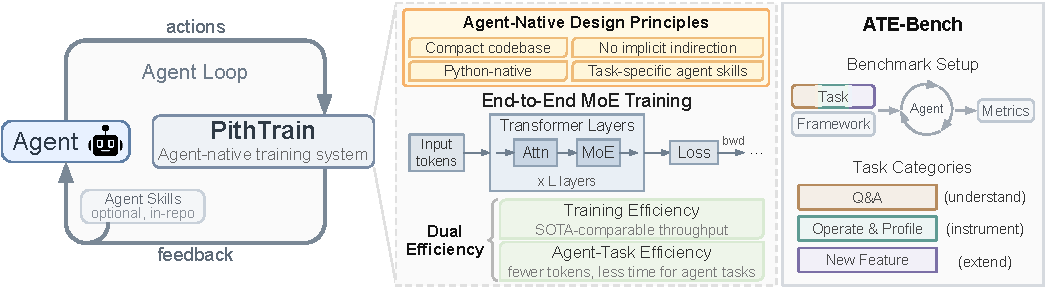
\includegraphics[width=0.95\textwidth]{figures/fig1_overview.pdf}
  \caption{\sys overview. An agent issues actions and consumes
  feedback (left); built on four agent-native design principles,
  \sys delivers dual efficiency (middle); \sysbench evaluates
  agent-task efficiency across frameworks (right).}
  \label{fig:overview}
\end{figure}

This paper makes three contributions:

\squishlist
    \item \textbf{\sys, a compact, Python-native, end-to-end MoE
    training framework.} A roughly 11K-line MoE training framework
    designed agent-native from the start, matching the training
    throughput of production frameworks.
    \vspace{-2pt}
    \item \textbf{Four design principles for agent-native ML
    training frameworks}, guiding \sys's design: code compactness,
    Python-native components, no implicit indirection, and agent
    skills.
    \vspace{-2pt}
    \item \textbf{Agent-task efficiency, \sysbench, and an
    empirical study.} Agent-task efficiency as a metric beyond
    training throughput, instantiated in \sysbench, with an
    empirical study showing
    \sys's higher agent-task efficiency over production frameworks,
    plus a skills ablation and case study.
\squishend

\sys delivers \emph{dual efficiency}: strong training throughput
together with high agent-task efficiency. It matches the throughput
of production frameworks across a range of MoE models and
training settings on NVIDIA H100 and B200 GPUs. On \sysbench, a
coding agent completes the same training-framework tasks on
\sys with up to 62\% fewer Agent Turns and 64\% less
Active GPU Time than on production frameworks
for the hardest new-feature tasks, with
similar reductions on other metrics. A qualitative case
study illustrates how framework design
shapes agent behavior.


\section{Related Work}
\label{sec:related}

Mature production frameworks have driven large-scale MoE training.
\megatron~\cite{shoeybi2020megatronlmtrainingmultibillionparameter,narayanan2021efficientlargescalelanguagemodel}
established the pipeline-parallel Transformer recipe most
subsequent frameworks build on, and
\deepspeed~\cite{deepspeed,rajbhandari2020zeromemoryoptimizationstraining}
introduced ZeRO sharded-optimizer techniques. Both rely on
layered designs with plugin systems, registry-based indirection,
and compiled extension chains, delivering broad model coverage
and peak throughput on production hardware.
\torchtitan~\cite{liang2025torchtitanonestoppytorchnative} more
recently scaled PyTorch-native training to multi-thousand-GPU
clusters, sharing \sys's Python-native goal but without making
agent-native design a primary axis or matching production-framework
throughput on our configurations. \sys takes a different point on
this tradeoff curve with agent-native design as a first-class
goal, achieving higher agent-task efficiency along Agent Turns,
Output Tokens, etc., while matching the training throughput of
production frameworks.

AI coding agents combine a tool-using language model with a small,
stable vocabulary of primitives (read, edit, shell, search).
Recent work designs better agent flows and harnesses for software
engineering on top of these
primitives~\cite{yao2023react,yang2024sweagentagentcomputerinterfacesenable,zhang2024autocoderoverautonomousprogramimprovement}.
\sys takes a complementary direction: rather than improving the
agent flow, we design the software framework so that existing
flows work better, lowering agent cost without changing the agent.

Existing agent benchmarks score capability on fixed codebases and
tasks: SWE-bench~\cite{jimenez2024swebench} on GitHub-issue
resolution, MLE-bench~\cite{chan2025mlebench} on Kaggle-style ML
engineering, and
HumanEval~\cite{chen2021evaluatinglargelanguagemodels} on
function-level code generation. Closer to ML systems engineering,
FlashInfer-Bench~\cite{xing2026flashinferbenchbuildingvirtuouscycle}
and KernelBench~\cite{ouyang2025kernelbench} target inference
operators and GPU kernels respectively. The agent is the variable;
aggregate task correctness is the metric. \sysbench inverts this: holding
the agent and task fixed, we vary the training framework so
that differences in agent cost and task outcome isolate framework
design. This axis is complementary to
existing capability benchmarks.

\section{The \sys System}
\label{sec:pithtrain}


\subsection{Agent-Native Design Principles}
\label{sec:pithtrain:principles}

This subsection introduces the four agent-native design principles
that guide \sys's system design, and contrasts how production
training frameworks align with each principle today.
\autoref{tab:principles-comparison} summarizes this comparison;
production frameworks adopt different subsets of the four
principles, reflecting different design priorities.

\begin{table}[t]
  \centering
  \small
  \caption{Adherence to agent-native design principles.
  \cmark{} satisfied; \pmark{} partial; \xmark{} not satisfied.
  Numbers are total framework LoC across Python, C++, and CUDA.\protect\footnotemark}
  \label{tab:principles-comparison}
  \begin{tabular}{lcccc}
    \toprule
    Framework & Compact & Python-native & No implicit indirection & Agent skills \\
    \midrule
    \megatron    & \xmark~149K  & \xmark & \xmark & \pmark \\
    \deepspeed   & \xmark~167K  & \xmark & \xmark & \xmark \\
    \torchtitan  & \pmark~38K   & \cmark & \pmark & \pmark \\
    \textbf{\sys} & \cmark~11K & \cmark & \cmark & \cmark \\
    \bottomrule
  \end{tabular}
\end{table}
\footnotetext{LoC measured at the pinned commits \texttt{3bec9aa}
(\megatron), \texttt{44c51e3} (\deepspeed), \texttt{d84e83d}
(\torchtitan), and \sys at v0.1.2.}


\MyPara{Compact codebase.}
Production frameworks such as \megatron and \deepspeed offer broad
coverage of models, training features, and hardware platforms,
accumulated over years of engineering effort, with core codebases
exceeding 160K lines. A larger codebase inflates the cost of
locating relevant code, tracking cross-file dependencies, and
verifying a change is complete. A compact codebase reduces this
cost; with frontier coding agents operating at context windows of
200K to 1M tokens, a sufficiently compact codebase can also fit in
a single context pass. We treat compactness as a constraint on
growth: \sys may grow over time, but additions should respect
the four principles.

\MyPara{Python-native codebase.}
Python is the dominant language in modern ML.
A pure-Python framework lets an agent navigate the full framework
in a single language, surfaces readable Python tracebacks instead
of opaque native errors, and eliminates the compiled-extension
rebuild cycle. \megatron composes its core transformer layers from
out-of-tree TransformerEngine~\cite{transformer-engine} modules,
and \deepspeed bundles extensive in-tree extensions. These deliver
peak kernel performance and vendor-tuned numerics, but push an
agent across language boundaries and force a rebuild on change.

\begin{figure}[t]
  \centering
  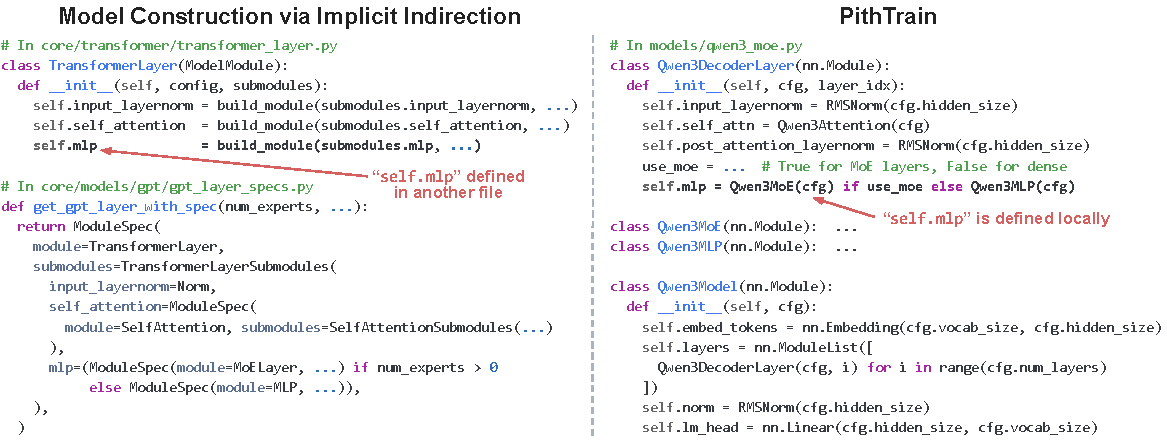
\includegraphics[width=0.9\textwidth]{figures/fig2_implicit_indirection.pdf}
\caption{Model construction patterns, illustrating the
  no-implicit-indirection principle. The implicit-indirection pattern
  resolves submodules through a runtime spec, supporting model
  variation from a shared layer skeleton; \sys instantiates
  layers directly, favoring local readability.}
  \label{fig:indirection-contrast}
\end{figure}

\MyPara{No implicit indirection.}
Production frameworks compose many model variants from a shared
layer skeleton via \emph{implicit indirection} (a stored
callable, plugin registry, or string-keyed resolution). This
pattern enables code reuse across models, while making what runs
at a given call site harder to identify by local reading.
\autoref{fig:indirection-contrast} shows an instance of model
construction in a production framework: \texttt{TransformerLayer}
resolves its submodules from a runtime spec in a separate file.
A flat code structure trades cross-model reuse for local
readability, reducing the effort an agent spends building an
end-to-end understanding.

\MyPara{Task-specific agent skills.}
An \emph{agent skill}~\cite{anthropic-skills} is a procedural
playbook a coding agent loads on demand. Skills encode procedural knowledge an agent cannot recover from static reading alone, so it
runs a verified procedure. Agent
skills are a recent practice that existing training frameworks
have not yet adopted at scale: \megatron ships six skills for
CI/PR hygiene; \torchtitan ships one
developer-workflow skill plus four editor rules orienting the
agent to the codebase; \deepspeed ships two markdown files with
generic rules. None of these target recurring training-framework
tasks.


\subsection{System Architecture and Optimizations}
\label{sec:pithtrain:arch-and-opt}

\begin{figure}[t]
\centering
\begin{minipage}[c]{0.58\textwidth}
  \centering
  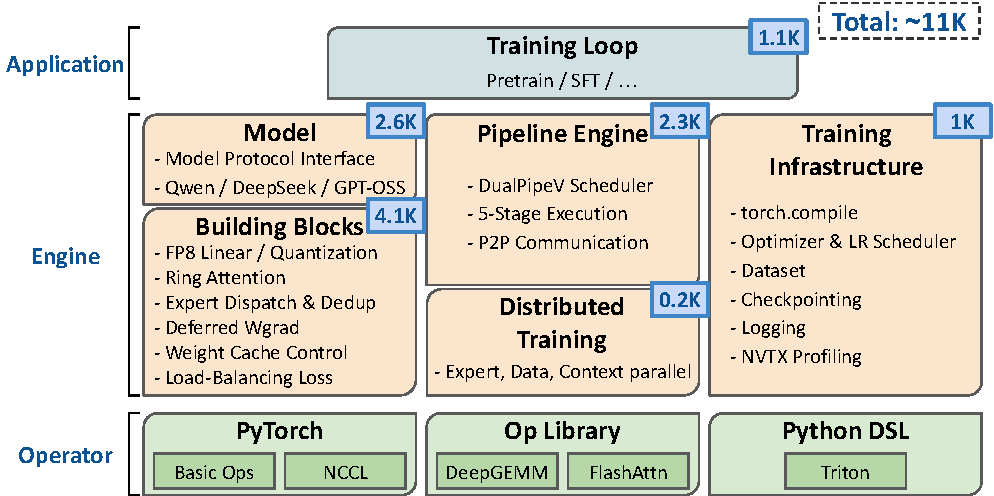
\includegraphics[width=\textwidth]{figures/fig3_architecture.pdf}
  \caption{\sys architecture with per-component line counts.}
  \label{fig:arch}
\end{minipage}%
\hfill
\begin{minipage}[c]{0.40\textwidth}
  \captionof{table}{Where \sys realizes each principle.}
  \label{tab:principle-map}
  \vspace{2pt}
  {\small
  \begin{tabular}{@{}>{\raggedright\arraybackslash}p{0.40\linewidth}@{\hspace{2pt}}>{\raggedright\arraybackslash}p{0.59\linewidth}@{}}
    \toprule
    Principle & Where it lives \\
    \midrule
    Compact codebase & All boxes in \autoref{fig:arch}; line counts sum to $\sim$11K \\
    \addlinespace
    Python-native codebase & Whole stack; Python-DSL for custom kernels only \\
    \addlinespace
    No implicit indirection & Whole codebase; flat structure \\
    \addlinespace
    Agent skills & Specialized skills under the project root \\
    \bottomrule
  \end{tabular}%
  }
\end{minipage}
\end{figure}

The codebase is organized in three layers (application, engine, operator), as shown in \autoref{fig:arch}.
To realize a compact codebase, we identified the necessary
components for a distributed MoE training framework, and \sys covers
exactly those. Where production
frameworks deliver broad out-of-the-box coverage of models,
features, and hardware, \sys narrows scope to keep the codebase
compact and reachable in a single context window.
Table~\ref{tab:principle-map} maps each principle to where it is
realized: we adopt a flat code structure with no plugin registries
or runtime specs, with each MoE model living in a self-contained
file under \texttt{models/} rather than being composed through a
shared layer skeleton. This favors local readability over cross-model
code reuse.

\sys supports standard MoE training\footnote{\sys also supports
dense (non-MoE) models, with MoE-specific machinery (e.g., expert
parallelism) skipped.} with pipeline parallelism (PP),
data parallelism (DP) via FSDP~\cite{pytorchfsdp}, context
parallelism (CP)~\cite{liu2024ringattention}, expert parallelism
(EP)~\cite{lepikhin2020gshardscalinggiantmodels}, FP8
training~\cite{micikevicius2022fp8formatsdeeplearning}, and DCP
checkpointing~\cite{torch-dcp}, on NVIDIA Hopper and Blackwell GPUs.
Despite its compact, Python-native codebase, \sys aims for
training throughput competitive with production frameworks by
adopting standard MoE optimizations; these techniques are not novel, but they are
central to \sys's training throughput and worth calling out.

\squishlist
\item \textbf{DualPipeV pipeline schedule and compute--communication overlap.}
\sys's pipeline scheduler builds on DualPipe from
DeepSeek-V3~\cite{deepseekai2025deepseekv3technicalreport}. DeepSeek's
open-source version provides a minimal pipeline-orchestration
scaffold, on top of which \sys implements the actual
compute--communication overlap. Each transformer layer is
decomposed into five stages at EP communication boundaries. EP
all-to-alls run on a separate communication stream, and the schedule
overlaps the forward of one micro-batch with the backward of another.

\vspace{-2pt}

\item \textbf{Torch compile.}
\sys applies \texttt{torch.compile(fullgraph=True)} to all
transformer computation except the MoE forward and backward. This
strict mode rejects graph breaks at compile time rather than
silently degrading speedup. We exclude the MoE forward and
backward because per-expert input shapes are data-dependent under
expert parallelism.

\vspace{-2pt}

\item \textbf{Other optimizations.}
\sys also implements
wgrad delay~\cite{qi2024zero}; fused SwiGLU~\cite{shazeer2020gluvariantsimprovetransformer} forward and
backward kernels for throughput and reduced activation memory; EP
dispatch deduplication for lower all-to-all communication volume;
an FP8 weight cache across micro-batches to avoid re-quantization;
and fused Triton kernels for EP token scatter and FP8 quantization.
\squishend


\subsection{Agent Skills}
\label{sec:pithtrain:skills}

A skill encodes the procedure for one recurring training-framework
task. \sys ships a suite of skills covering several common ones
(Table~\ref{tab:skills}). Each skill is a self-contained folder with
a top-level \texttt{SKILL.md} playbook, optionally additional markdown
documents, and optionally helper scripts. Some skills are pure
markdown, like \texttt{add-new-model}; others bundle scripts that
offload deterministic work.

\begin{figure}[t]
\centering
\begin{minipage}[c]{0.48\textwidth}
  \captionof{table}{Representative skills in \sys.}
  \label{tab:skills}
  \vspace{2pt}
  {\small
  \begin{tabular}{@{}p{0.32\linewidth}@{\hspace{6pt}}>{\raggedright\arraybackslash}p{0.60\linewidth}@{}}
    \toprule
    Skill & Purpose \\
    \midrule
    \texttt{add-\allowbreak{}new-\allowbreak{}model} & Port a new MoE architecture end-to-end (model, FSDP, tests) \\
    \addlinespace
    \texttt{add-\allowbreak{}memory-\allowbreak{}prints} & Instrument training for memory profiling \\
    \addlinespace
    \texttt{capture-\allowbreak{}nsys-\allowbreak{}profile} & Capture an Nsight Systems profile of a short \sys run \\
    \addlinespace
    \texttt{validate-\allowbreak{}correctness} & Compare per-step loss curves between branches \\
    \bottomrule
  \end{tabular}%
  }
\end{minipage}%
\hfill
\begin{minipage}[c]{0.48\textwidth}
  \centering
  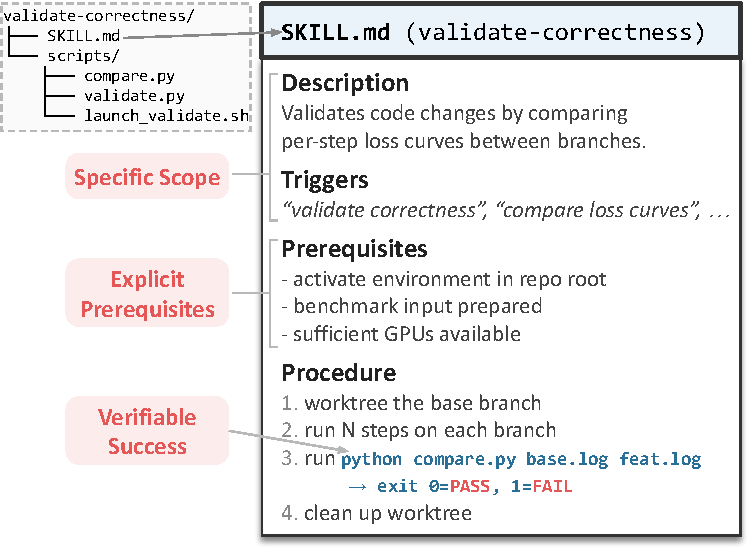
\includegraphics[width=0.95\textwidth]{figures/fig4_skill}
  \caption{The \texttt{validate-correctness} skill in \sys. Pink labels mark properties.}
  \label{fig:skill-anatomy}
\end{minipage}
\vspace{-10pt}
\end{figure}

Each skill in \sys is designed around three properties:
\emph{specific scope}, \emph{explicit prerequisites}, and
\emph{verifiable success}. \autoref{fig:skill-anatomy} illustrates
these on \texttt{validate-correctness}. The description and triggers
together encode the skill's specific scope. The prerequisites section
enumerates environment, data, and configuration assumptions, so
missing state is caught before the skill begins to run. The procedure
ends in a script call that returns a reproducible PASS/FAIL verdict
rather than the agent's self-assessment. Skills designed around these
properties are not technically hard to author, and we expect other
training frameworks to ship comparable coverage as the practice
matures.
\section{\sysbench: A Benchmark for Agent-Task Efficiency}
\label{sec:benchmark}




Evaluating the agent-task efficiency of a training framework requires
varying the framework while holding the agent and task fixed. This is
the inverse of standard benchmarks for AI coding agents~\cite{jimenez2024swebench,chen2021evaluatinglargelanguagemodels,austin2021programsynthesislargelanguage},
which hold the codebase and task fixed and vary the agent to score
capability. We introduce \sysbench,
a benchmark with a fixed agent and curated task suite run across
frameworks, so that differences in agent performance are
attributable to framework design. The suite spans the kinds of work
researchers typically perform on training frameworks, organized
around three recurring patterns: understanding the framework
without modifying it, operating it as a tool for instrumentation
and profiling, and extending it with new functionality. Tasks are distributed across three categories:
\squishlist
  \vspace{-3pt}
  \item Q\&A (12 tasks): answer questions whose answer is a
  property of the code, not a runtime measurement (e.g., ``how is
  the device mesh built?'').
  \vspace{-3pt}
  \item Operate and Profile (4 tasks): run, instrument, and
  profile the framework as a tool (e.g., capture an Nsight Systems
  profile and identify the most expensive CUDA kernels).
  \vspace{-3pt}
  \item New Feature (4 tasks): port a new model architecture into
  the framework end-to-end against a published reference
  implementation (e.g., Mixture of Block Attention
  (MoBA)~\cite{lu2025moba}).
  \vspace{-3pt}
\squishend


\autoref{fig:benchmark-harness} illustrates the agent loop for each
category, with agent involvement deepening from Q\&A (read-only)
to Operate and Profile (running, minor instrumentation) to New
Feature (substantial modification, test-driven iteration). Full
task descriptions and per-category correctness checks are in
Appendix~\ref{sec:appendix:tasks}. Using \sysbench, we evaluate
\sys and production frameworks, reporting five effort metrics:
session duration, active GPU time, agent turns, per-turn context,
and output tokens. Without a single-scalar metric for agent-task
efficiency, we report each dimension independently.

Q\&A questions are chosen to be valid across all three
frameworks, excluding framework-specific behaviors.
\sysbench does not cover tasks like cross-model propagation of
a shared change, where production frameworks' implicit
indirection may lower agent effort; we leave these as future work.

\begin{figure}[t]
  \centering
  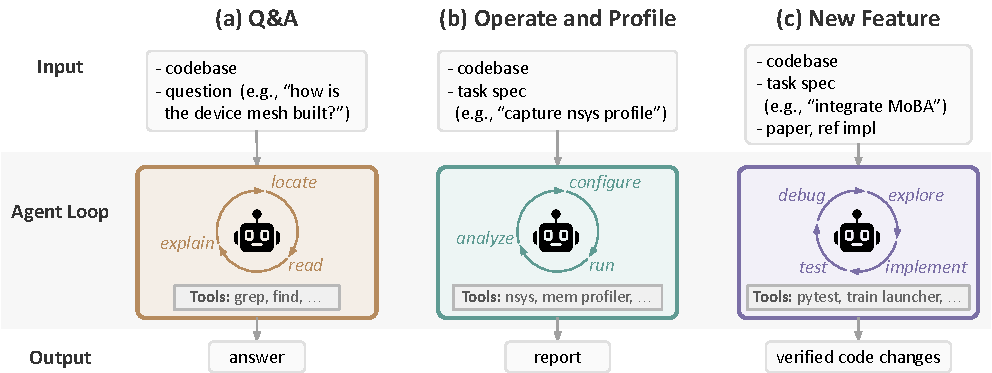
\includegraphics[width=0.85\textwidth]{figures/fig5_agent_loop.pdf}
  \caption{Per-category agent loop. Steps, tools, and output differ across categories.
  }
  \vspace{-9pt}
  \label{fig:benchmark-harness}
\end{figure}

\section{Evaluation}
\label{sec:evaluation}

We evaluate \sys on both axes of dual efficiency: training
efficiency and agent-task efficiency. We validate training
correctness against \megatron on both pretraining loss curves and
downstream accuracy in
Appendix~\ref{sec:appendix:model-quality}.
This section is organized to answer the following questions:
\squishlist
  \vspace{-2pt}
  \item Does \sys deliver competitive training throughput against production frameworks?~(\S\ref{sec:eval:training})
  \vspace{-2pt}
  \item Does \sys offer higher agent-task efficiency than production frameworks?~(\S\ref{sec:eval:agent})
  \vspace{-2pt}
  \item How much do agent skills improve agent-task efficiency on \sys?~(\S\ref{sec:eval:skills-ablation})
  \vspace{-2pt}
  \item Where do the per-framework differences in agent cost come from
  on a single concrete task?~(\S\ref{sec:eval:case})
  \vspace{-2pt}
\squishend

\subsection{Training Efficiency}
\label{sec:eval:training}







\begin{table}[t]
  \centering
  \small
  \caption{Training throughput across frameworks.
  We report the aggregate tokens per second as the training throughput.
  ``---'' denotes not supported; ``OOM'' denotes out of memory.
  }
  \label{tab:training-throughput}
  \setlength{\tabcolsep}{3pt}
  \begin{tabular}{lll|ccc}
    \toprule
    Model & Hardware & Parallelism / SeqLen / Precision & \megatron & \torchtitan & \sys \\
    \midrule
    GPT-OSS-20B      & 1$\times$8-B200 & PP2,DP1,CP1,EP4 / 8192 / BF16 & 129.5K & ---\protect\footnotemark{} & 140.9K \\
    Qwen3-30B-A3B    & 1$\times$8-B200 & PP2,DP1,CP1,EP4 / 8192 / FP8  & 106.2K & OOM & 134.5K \\
    Qwen3-30B-A3B    & 2$\times$8-H100 & PP2,DP1,CP1,EP8 / 2048 / BF16 & 126.7K & 90.5K  & 124.9K \\
    Qwen3-30B-A3B    & 4$\times$8-H100 & PP4,DP1,CP1,EP8 / 4096 / BF16 & 264.1K & OOM & 280.0K \\
    DeepSeek-V2-Lite & 1$\times$8-H100 & PP2,DP1,CP1,EP4 / 2048 / BF16 & 107.3K & 74.1K  & 114.6K \\
    \bottomrule
  \end{tabular}
\end{table}
\footnotetext{\torchtitan does support GPT-OSS-20B training, but not with pipeline parallelism.}

We compare \sys~(\texttt{23db182}), \megatron~\cite{narayanan2021efficientlargescalelanguagemodel}~(\texttt{3bec9aa})
and \torchtitan~\cite{liang2025torchtitanonestoppytorchnative}~(\texttt{d84e83d}) on three
representative MoE models (GPT-OSS-20B~\cite{openai2025gptoss120bgptoss20bmodel},
Qwen3-30B-A3B~\cite{yang2025qwen3technicalreport}, and
DeepSeek-V2-Lite~\cite{deepseekai2024deepseekv2strongeconomicalefficient})
under matched parallelism (PP, DP, CP, EP), sequence length, and precision.
Configurations span single-node and multi-node deployments on
NVIDIA H100 and B200 GPUs.
For \megatron, we follow NVIDIA's documented best practices\protect\footnote{\url{https://docs.nvidia.com/nemo/megatron-bridge/nightly/training/moe-optimization.html}}.
\deepspeed is excluded as it does not currently support PP combined with EP for MoE
training\protect\footnote{Verified at commit \texttt{44c51e3}: the
Megatron-DeepSpeed integration script states ``Currently we don't
support PP for MoE.''}, so it cannot run any of the configurations in
our suite.

To ensure the MoE router exhibits steady-state load-balanced
routing across frameworks and thus comparable throughput,
we load public model checkpoints rather than random initializations.
Each experiment runs 25 steps, and we report the median step
time over the last 10. We omit Model FLOPs Utilization
(MFU)~\cite{chowdhery2023palm} because Tensor Core peak FLOPS differs
between BF16 and FP8, making the metric ambiguous for 
mixed-precision steps.
Training hyperparameters follow
Appendix~\ref{sec:appendix:model-quality}.

As \autoref{tab:training-throughput} shows, \sys matches or exceeds
\megatron on 4 of 5 configurations, and stays within 1.4\% of
\megatron on the fifth. This parity comes from optimizations such
as DualPipeV's compute--communication overlap and
\texttt{torch.compile(fullgraph=True)}. These results demonstrate
that a compact, Python-native codebase can achieve competitive
training throughput.

\subsection{Agent-Task Efficiency}
\label{sec:eval:agent}

In this section, we evaluate agent-task efficiency across
frameworks.
We run \sysbench (\S\ref{sec:benchmark}) on \megatron, \torchtitan,
and \sys with Claude Code (Opus~4.7 at
\texttt{xhigh} effort\protect\footnote{\url{https://platform.claude.com/docs/en/build-with-claude/effort}})
as the fixed agent. Each task runs three times and we report
medians; hardware configuration, task descriptions, correctness criteria, and per-attempt
values are described in Appendix~\ref{sec:appendix:tasks} and
\ref{sec:appendix:per-task-results}. Opus~4.7 completed
every task across all attempts and frameworks with no failure.

\MyPara{Q\&A.}
Answering a question requires locating where a behavior lives in
the codebase. We omit Session Duration (all tasks finish in under
three minutes) and Active GPU Time (no training runs). All 12
questions are answered correctly across attempts and frameworks
(grading details in
Appendix~\ref{sec:appendix:tasks:qa-correctness}).
Across the 12 questions, the agent uses up to 67\% fewer Agent Turns to reach the final answer on \sys than on \megatron.
A compact codebase and the
absence of implicit indirection shrink the search space, lowering
Per-Turn Context (\autoref{tab:agent-efforts-codebaseqa})
accordingly.

\begin{table}[t]
  \centering
  \small
  \vspace{-7pt}
  \caption{Per-question agent effort on the Q\&A task suite
  (\S\ref{sec:benchmark}); Q1--Q12 are described in
  Appendix~\ref{sec:appendix-codebaseqa}. Each metric reports the
  median of three independent attempts. Lower is more efficient.
  Headers abbreviate \megatron, \torchtitan, and \sys.}
  \label{tab:agent-efforts-codebaseqa}
  \begin{tabular}{c|rrr|rrr|rrr}
    \toprule
       & \multicolumn{3}{c|}{Agent Turns}    & \multicolumn{3}{c|}{Per-Turn Context}            & \multicolumn{3}{c}{Output Tokens} \\
    \# & Megatron & Titan & Pith & Megatron & Titan & Pith & Megatron & Titan & Pith \\
    \midrule
    Q1  & 33         & 18          & \textbf{15} & 45.8K          & 44.3K          & \textbf{33.4K} & 9.0K           & 7.1K           & \textbf{4.1K}  \\
    Q2  & 54         & 28          & \textbf{18} & 41.2K          & 43.5K          & \textbf{35.9K} & 10.7K          & 7.8K           & \textbf{5.4K}  \\
    Q3  & 14         & 14          & \textbf{13} & \textbf{31.3K} & 36.1K          & 34.1K          & \textbf{3.4K}  & 3.5K           & 3.4K           \\
    Q4  & 36         & 26          & \textbf{16} & 41.3K          & 39.7K          & \textbf{31.1K} & 10.0K          & 6.9K           & \textbf{5.2K}  \\
    Q5  & 48         & \textbf{19} & 21          & 46.5K          & 41.7K          & \textbf{33.8K} & 10.7K          & 4.8K           & \textbf{4.6K}  \\
    Q6  & 12         & \textbf{4}  & 11          & 36.4K          & 29.9K          & \textbf{27.9K} & 4.5K           & \textbf{2.3K}  & 3.3K           \\
    Q7  & \textbf{9} & 12          & 14          & 31.5K          & \textbf{30.0K} & 31.5K          & \textbf{2.6K}  & 3.4K           & 4.2K           \\
    Q8  & 20         & 11          & \textbf{9}  & 30.8K          & 32.7K          & \textbf{28.7K} & 4.7K           & 3.5K           & \textbf{3.2K}  \\
    Q9  & 34         & \textbf{16} & \textbf{16} & 45.2K          & 38.6K          & \textbf{37.0K} & 7.6K           & 6.0K           & \textbf{5.1K}  \\
    Q10 & 19         & 17          & \textbf{11} & 37.8K          & 38.8K          & \textbf{29.4K} & 5.9K           & 5.1K           & \textbf{2.9K}  \\
    Q11 & 10         & 8           & \textbf{6}  & 31.3K          & 30.1K          & \textbf{25.6K} & 3.1K           & 2.5K           & \textbf{2.0K}  \\
    Q12 & 18         & \textbf{5}  & 10          & 37.1K          & 33.9K          & \textbf{31.1K} & 5.1K           & \textbf{2.2K}  & 2.6K           \\
    \bottomrule
  \end{tabular}
\end{table}

\MyPara{Operate and Profile.}
Across all tasks (\autoref{tab:agent-efforts-operate}), \sys's Agent Turns are up to 70\% lower than \megatron's and 57\% lower than \torchtitan's, and its Output Tokens are up to 78\% and 65\% lower respectively.
\sys's compact codebase explains these reductions.
In addition, the agent invokes in-repo
skills (\S\ref{sec:pithtrain:skills}) on its own when applicable;
for example, the \emph{Report Heavy Kernels} task triggers
\texttt{capture-nsys-profile}.

\begin{table}[t]
  \centering
  \small
  \caption{Per-task agent effort across frameworks on
  operate-and-profile tasks (\S\ref{sec:benchmark}). Each metric
  reports the median of three independent attempts. Lower is more
  efficient. Session Duration and Active GPU Time are in minutes. Per-attempt metrics in Appendix~\ref{sec:appendix:per-task-results}.}
  \label{tab:agent-efforts-operate}
  \setlength{\tabcolsep}{3pt}
  \begin{tabular}{@{}lr|rrrrr@{}}
    \toprule
    Task
      & Framework
      & \makecell[br]{Session\\Duration}
      & \makecell[br]{Active\\GPU Time}
      & \makecell[br]{Agent\\Turns}
      & \makecell[br]{Per-Turn\\Context}
      & \makecell[br]{Output\\Tokens} \\
    \midrule
    \multirow{3}{*}{\textit{Getting Started}}
      & \megatron   & 40.5 &  5.4 &  88 &  69.5K & 26.9K \\
      & \torchtitan & 11.4 &  5.2 &  54 &  56.8K & 15.8K \\
      & \sys        & \textbf{6.6} & \textbf{3.1} & \textbf{26} & \textbf{37.0K} & \textbf{5.8K} \\
    \midrule
    \multirow{3}{*}{\textit{Train and Evaluate}}
      & \megatron   & 55.5 & 36.0 & 163 & 106.4K & 52.9K \\
      & \torchtitan & 72.5 & 36.3 & 212 & 176.6K & 97.8K \\
      & \sys        & \textbf{38.5} & \textbf{22.7} & \textbf{92} & \textbf{85.5K} & \textbf{34.2K} \\
    \midrule
    \multirow{3}{*}{\textit{Collect Routing Trace}}
      & \megatron   & 33.3 &  5.5 & 112 & 144.3K & 102.1K \\
      & \torchtitan & 32.8 & 10.4 & 103 & 166.0K &  84.7K \\
      & \sys        & \textbf{16.3} & \textbf{2.8} & \textbf{58} & \textbf{118.7K} & \textbf{56.2K} \\
    \midrule
    \multirow{3}{*}{\textit{Report Heavy Kernels}}
      & \megatron   & 22.1 & 12.1 & 60 & 52.6K & 23.9K \\
      & \torchtitan & 15.0 &  6.7 & \textbf{40} & 66.1K & 22.5K \\
      & \sys        & \textbf{11.8} & \textbf{3.6} & 42 & \textbf{49.2K} & \textbf{16.0K} \\
    \bottomrule
  \end{tabular}
\end{table}

\MyPara{New Feature.}
New-feature tasks exercise the test--debug cycle: edit, run
training, read crash, edit again.
Across all tasks (\autoref{tab:agent-efforts}), \sys's Active GPU Time is up to 44\% lower than \megatron's and 64\% lower than \torchtitan's, primarily because \sys converges in fewer training runs.
Two patterns inflate \megatron's reruns: a hidden argument
registry causes the agent's manually-added CLI flags to collide
with auto-derived ones (implicit indirection), and C++ paths like
TransformerEngine's grouped-GEMM emit opaque segfaults that drive
speculative configuration toggles (not Python-native).
\torchtitan's reruns are dominated by memory-pressure debugging.
On \sys, failures surface inside the file the agent just wrote
with a readable Python traceback, and fixes stay in the same
file. \S\ref{sec:eval:case} provides a detailed case study on
MoBA.

\begin{table}[t]
  \centering
  \small
  \vspace{-5pt}
  \caption{Per-task agent effort across frameworks on new-feature
  tasks (\S\ref{sec:benchmark}). Each metric reports the median of
  three independent attempts. Lower is more efficient. Session Duration
  and Active GPU Time are in minutes. Per-attempt metrics in
  Appendix~\ref{sec:appendix:per-task-results}.
  }
  \label{tab:agent-efforts}
  \setlength{\tabcolsep}{3pt}
  \begin{tabular}{@{}lr|rrrrr@{}}
    \toprule
    Task
      & Framework
      & \makecell[br]{Session\\Duration}
      & \makecell[br]{Active\\GPU Time}
      & \makecell[br]{Agent\\Turns}
      & \makecell[br]{Per-Turn\\Context}
      & \makecell[br]{Output\\Tokens} \\
    \midrule
    \multirow{3}{*}{\makecell[l]{\textit{Differential Transformer}\\(Diff)~\cite{ye2024differential}}}
      & \megatron   & 47.1 & 33.7 & 125 & 118.7K & 57.1K \\
      & \torchtitan & 49.6 & 40.3 &  58 & 103.2K & 36.0K \\
      & \sys        & \textbf{38.2} & \textbf{27.6} & \textbf{47} & \textbf{69.5K} & \textbf{25.4K} \\
    \midrule
    \multirow{3}{*}{\makecell[l]{\textit{Dynamic Mixture of Experts}\\(DynMoE)~\cite{guo2024dynamic}}}
      & \megatron   &  83.8 & 49.1 & 199 & 208.0K & 115.2K \\
      & \torchtitan & 140.6 & 94.4 & 197 & 228.8K & 161.3K \\
      & \sys        & \textbf{60.4} & \textbf{41.9} & \textbf{76} & \textbf{146.0K} & \textbf{76.4K} \\
    \midrule
    \multirow{3}{*}{\makecell[l]{\textit{Mixture of Block Attention}\\(MoBA)~\cite{lu2025moba}}}
      & \megatron   &  61.6 & 49.5 & 134 & 120.9K &  53.8K \\
      & \torchtitan & 105.1 & 77.9 &  91 & 166.9K & 111.8K \\
      & \sys        & \textbf{38.7} & \textbf{27.7} & \textbf{57} & \textbf{69.0K} & \textbf{32.4K} \\
    \midrule
    \multirow{3}{*}{\textit{MoE++}~\cite{jin2025moeplusplus}}
      & \megatron   & 88.5 & 58.7 & 145 & 188.7K & 117.0K \\
      & \torchtitan & 71.4 & 51.9 & \textbf{87} & \textbf{164.6K} & \textbf{85.3K} \\
      & \sys        & \textbf{63.0} & \textbf{39.9} &  90 & 176.6K & 107.7K \\
    \bottomrule
  \end{tabular}
\end{table}


\subsection{Ablation Study on Agent Skills}
\label{sec:eval:skills-ablation}



In this section, we isolate the effect of agent skills via
ablation. They are a self-contained set of files shipped in the
repository, so we can toggle them on and off against an otherwise
fixed codebase. We
pick two of
\sys's skills, \texttt{validate-correctness} and
\texttt{capture-nsys-profile}, which mirror the natural follow-up
after a system optimization: validate that training correctness is
preserved, then capture an Nsight Systems profile to examine
whether the optimization is effective.

We run this ablation on the wgrad delay~\cite{qi2024zero} commit in
\sys, repeating each task three times with skills and three times
without. The codebase, agent, and harness are otherwise identical,
and we report the same five effort metrics as in
\S\ref{sec:eval:agent}. When skills are disabled, we strip them
from both the working tree and the git history, so the agent cannot
recover the procedure from either. All twelve runs completed
successfully, reporting the correct verdict or generating a valid
Nsight Systems profile.

\autoref{tab:skills-ablation} reports the results. Active GPU
Time stays near parity across both tasks: each task runs a fixed
set of training runs pinned by the workflow, so the GPU work is
determined by the task rather than the agent. The four agent-side
metrics, which capture the agent's reasoning overhead in setup,
launch, and interpretation, all drop substantially with skills
enabled. Agent turns drop the most (70\% and 52\% respectively),
suggesting that with the procedure encoded in the skill, the agent
acts on a fixed plan rather than iteratively deriving one through
repeated tool calls. These results demonstrate that task-specific
in-repo skills, comprising the markdown playbook and any helper
scripts, substantially reduce agent effort on the recurring
training-system tasks they target.





\begin{table}[t]
  \centering
  \small
  \caption{Agent effort on \sys with and without the corresponding
  skill. Each metric reports the median of three independent
  attempts. Session Duration and Active GPU Time are in minutes.}
  \label{tab:skills-ablation}
  \setlength{\tabcolsep}{3pt}
  \begin{tabular}{@{}lr|rrrrr@{}}
    \toprule
    Task
      & Skills
      & \makecell[br]{Session\\Duration}
      & \makecell[br]{Active\\GPU Time}
      & \makecell[br]{Agent\\Turns}
      & \makecell[br]{Per-Turn\\Context}
      & \makecell[br]{Output\\Tokens} \\
    \midrule
    \multirow{2}{*}{\texttt{validate-correctness}}
      & off & 26.0 & 20.8 & 114 & 96.3K & 30.2K \\
      & on  & 22.9 & 22.5 &  34 & 43.5K & 11.3K \\
    \midrule
    \multirow{2}{*}{\texttt{capture-nsys-profile}}
      & off &  9.4 &  5.6 &  75 & 62.1K & 25.3K \\
      & on  &  6.6 &  5.5 &  36 & 40.3K & 14.5K \\
    \bottomrule
  \end{tabular}
\end{table}

\subsection{Case Study: Integrating MoBA}
\label{sec:eval:case}




\begin{figure}[t]
  \centering
  \begin{subfigure}[t]{0.45\linewidth}
    \centering
    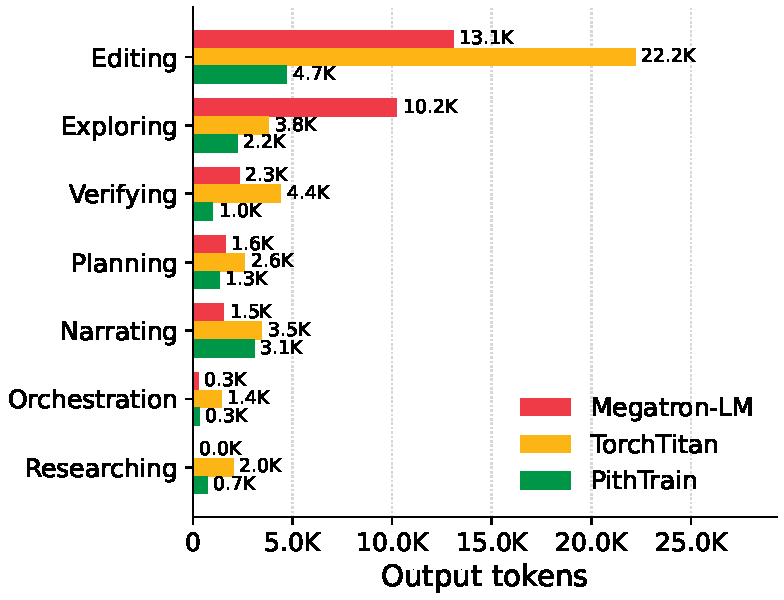
\includegraphics[width=\linewidth]{figures/token_breakdown.pdf}
    \caption{Per-category breakdown of output tokens.}
    \label{fig:moba-token-breakdown}
  \end{subfigure}
  \hfill
  \begin{subfigure}[t]{0.45\linewidth}
    \centering
    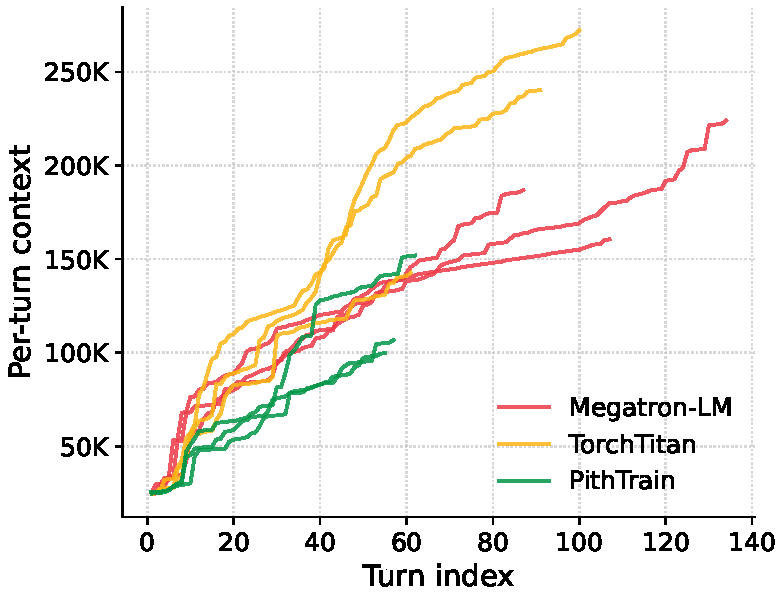
\includegraphics[width=\linewidth]{figures/context_trace.pdf}
    \caption{Per-turn context window over the session.}
    \label{fig:moba-context-trace}
  \end{subfigure}
  \caption{Agent behavior on integrating MoBA across frameworks.
  (\subref{fig:moba-token-breakdown}) reports the median output
  tokens per action category of three independent attempts;
  (\subref{fig:moba-context-trace}) shows the per-turn input-side
  context for each of three independent attempts.}
  \label{fig:moba-case-figures}
\end{figure}


To examine where per-framework differences in agent cost come from,
we conduct a case study on integrating MoBA, decomposing the
agent's output tokens by action
category\footnote{Thinking tokens are excluded as they are not
surfaced by the API.}~(\autoref{fig:moba-token-breakdown}) and
tracing its per-turn context
window~(\autoref{fig:moba-context-trace}). Editing dominates
across all three frameworks (\sys 4.7K, \megatron 13.1K,
\torchtitan 22.2K). \megatron also spends substantially more on
Exploring (10.2K vs.\ 3.8K for \torchtitan and 2.2K for \sys),
and its per-turn context sits well above \sys's. The agent reads
the codebase to locate edits and interpret tracebacks, so a
compact codebase with no implicit indirection lowers both
Exploring and per-turn context. \torchtitan's elevated Editing
and \textasciitilde2$\times$ context spike in two of three runs have a different
cause: the agent's initial implementation runs out of memory
(OOM), forcing repeated debug-edit cycles. This points to runtime
properties like memory headroom as a factor independent of
codebase structure.

Beyond \torchtitan's memory failures, we examine the other
failures the agent encountered. Across the three \sys runs, two
complete without any failure; the third hits a tensor-stride
mismatch in the agent's custom attention kernel, fixed in the same
file as the traceback. \megatron's three runs hit two distinct failures: two runs fail
with a duplicate command-line flag registration that conflicts with
one defined in framework code, and one run fails with a BF16
overflow in the agent's code. Each fix on \megatron spans multiple
files. This
contrast reflects \sys's compactness and absence of implicit
indirection, which keep each fix local to the agent's edit.





\section{Conclusion}
\label{sec:conclusion}

We presented \sys, a compact, agent-native MoE training framework
built on four design principles.
\sys matches the throughput of production frameworks across a
range of models, and on \sysbench, a coding agent achieves higher
agent-task efficiency on \sys than on production frameworks.
We hope \sys serves as a starting point for future agent-native
training framework.



\begin{ack}
\sys is developed by contributors from CMU. We thank the CMU Foundation and
Language Model (FLAME) Center for providing the compute resources to develop
\sys. We also acknowledge the support of DGX B200 from NVIDIA.
\end{ack}


\bibliography{reference}
\bibliographystyle{plain}


\clearpage
\appendix

\section{Training Correctness}
\label{sec:appendix:model-quality}

This appendix validates the training correctness of \sys against
\megatron at matched configuration.
We report two complementary measurements: pretraining loss
trajectories (\S\ref{sec:appendix:loss-curve}) and downstream task
accuracy (\S\ref{sec:appendix:downstream}).

\subsection{Pretraining Loss}
\label{sec:appendix:loss-curve}

We pretrain Qwen3-30B-A3B with \megatron and \sys under identical
configuration. \autoref{fig:appendix-loss-curve} reports the full
training configuration alongside the two loss curves; the
trajectories align across the full run, with \megatron showing two
transient spikes that recover within a few steps.

\begin{figure}[t]
  \centering
  \begin{minipage}[c]{0.36\linewidth}
    \centering
    \footnotesize
    \setlength{\tabcolsep}{4pt}
    \begin{tabular}{ll}
      \toprule
      Hardware       & 4$\times$8-H100 \\
      Parallelism    & PP4, DP1, CP1, EP8 \\
      Dataset        & DCLM~\cite{li2024dclm} \\
      Sequence       & 2048 \\
      Precision      & BF16 \\
      Global Batch   & 1024 \\
      Training Steps & 4096 \\
      Warmup Steps   & 128 \\
      Optimizer      & Adam~\cite{kingma2015adam} \\
      Max LR         & $2\times10^{-4}$ \\
      Min LR         & $1\times10^{-5}$ \\
      LR Schedule    & Cosine Decay \\
      Aux Loss       & Global-Level~\cite{qiu2025demonsdetailimplementingload} \\
      Aux Coef       & $1\times10^{-3}$ \\
      \bottomrule
    \end{tabular}
  \end{minipage}
  \hfill
  \begin{minipage}[c]{0.62\linewidth}
    \centering
    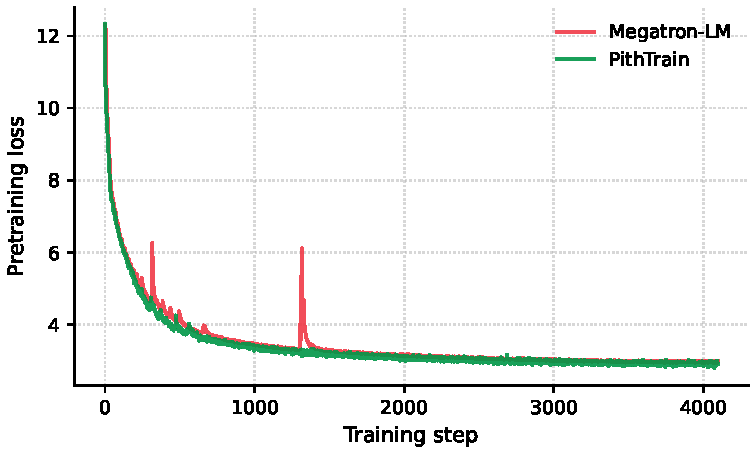
\includegraphics[width=\linewidth]{figures/loss_curve.pdf}
  \end{minipage}
  \caption{Training configuration (left) and pretraining loss curves
  (right) for Qwen3-30B-A3B trained with \megatron and \sys.}
  \label{fig:appendix-loss-curve}
\end{figure}

\subsection{Downstream Accuracy}
\label{sec:appendix:downstream}

We evaluate downstream task accuracy across six standard
benchmarks:
OpenBookQA~\cite{mihaylov2018openbookqa} and
WinoGrande~\cite{sakaguchi2020winogrande} in the 0-shot setting, and
ARC-Challenge, ARC-Easy~\cite{clark2018arc},
HellaSwag~\cite{zellers2019hellaswag}, and PIQA~\cite{bisk2020piqa} in
the 10-shot setting. \autoref{fig:appendix-downstream} plots
accuracy for each task; \megatron and \sys achieve comparable
accuracy within statistical noise across all six benchmarks at every
checkpoint.

\begin{figure}[t]
  \centering
  \begin{subfigure}{0.32\linewidth}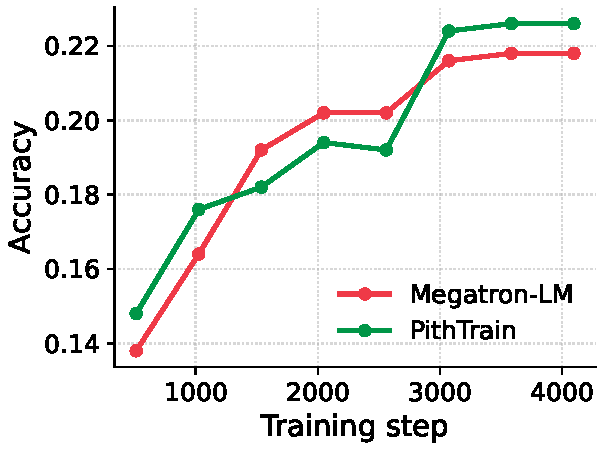
\includegraphics[width=\linewidth]{figures/downstream_openbookqa.pdf}\caption{OpenBookQA (0-shot)}\end{subfigure}
  \hfill
  \begin{subfigure}{0.32\linewidth}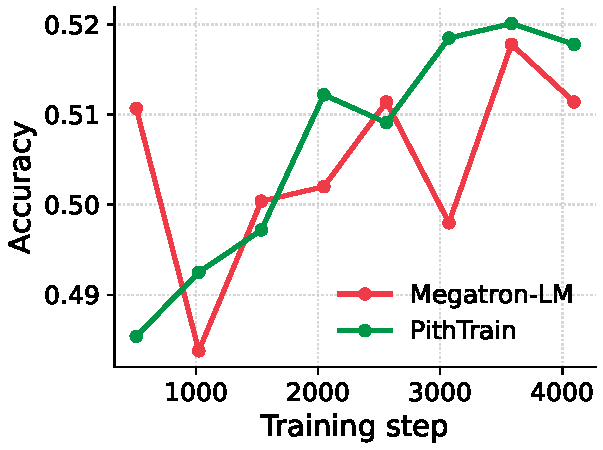
\includegraphics[width=\linewidth]{figures/downstream_winogrande.pdf}\caption{WinoGrande (0-shot)}\end{subfigure}
  \hfill
  \begin{subfigure}{0.32\linewidth}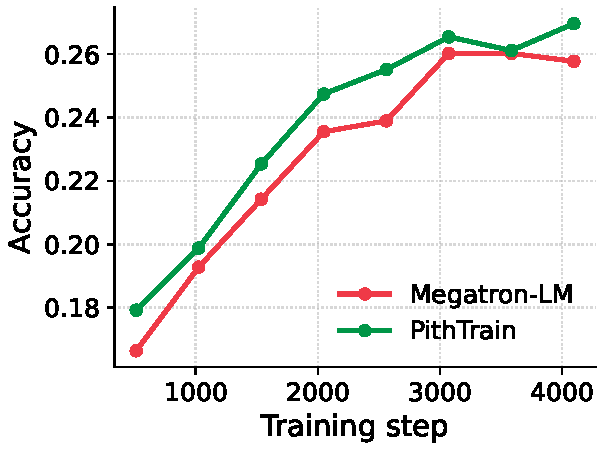
\includegraphics[width=\linewidth]{figures/downstream_arc_challenge.pdf}\caption{ARC-Challenge (10-shot)}\end{subfigure}

  \medskip
  \begin{subfigure}{0.32\linewidth}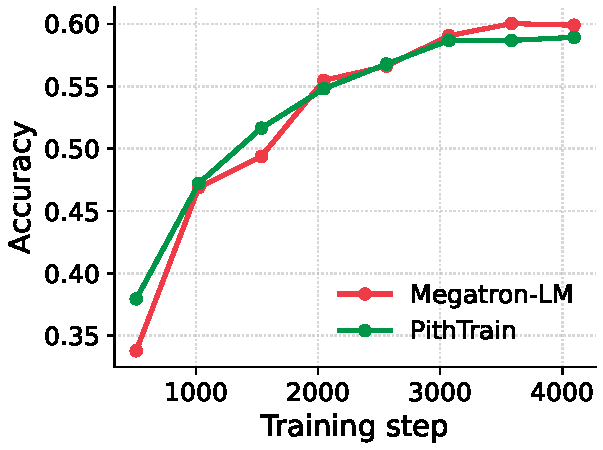
\includegraphics[width=\linewidth]{figures/downstream_arc_easy.pdf}\caption{ARC-Easy (10-shot)}\end{subfigure}
  \hfill
  \begin{subfigure}{0.32\linewidth}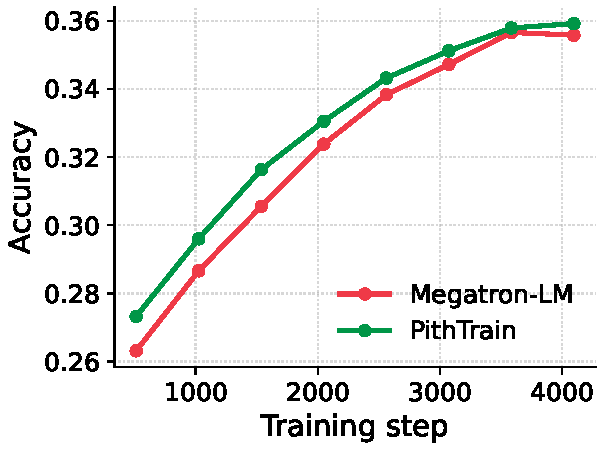
\includegraphics[width=\linewidth]{figures/downstream_hellaswag.pdf}\caption{HellaSwag (10-shot)}\end{subfigure}
  \hfill
  \begin{subfigure}{0.32\linewidth}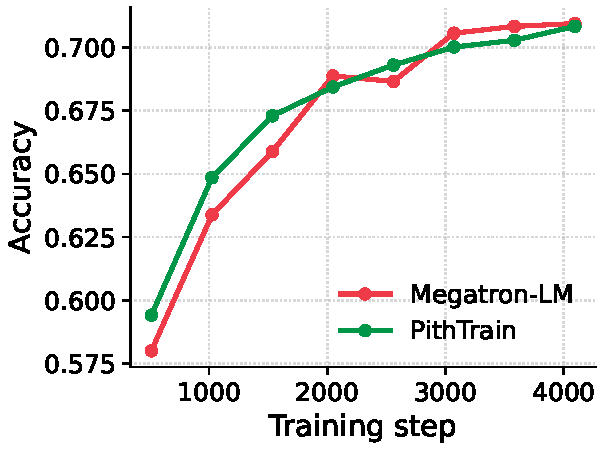
\includegraphics[width=\linewidth]{figures/downstream_piqa.pdf}\caption{PIQA (10-shot)}\end{subfigure}

  \caption{Downstream task accuracy for Qwen3-30B-A3B trained with
  \megatron and \sys.}
  \label{fig:appendix-downstream}
\end{figure}


\section{Task Suite}
\label{sec:appendix:tasks}

This appendix expands the per-category task descriptions and the
correctness checks used to validate each attempt. All
operate-and-profile and new-feature tasks share a fixed training
configuration: the base model is
DeepSeek-V2-Lite~\cite{deepseekai2024deepseekv2strongeconomicalefficient}
(its training fits within a single node with 8 NVIDIA H100 GPUs), the
parallelism mesh is PP=4, EP=2, DP=1, sequence length 2048, global
batch size 1024, precision BF16.

\subsection{Q\&A Tasks}
\label{sec:appendix-codebaseqa}

Each Q\&A task asks the agent to locate where a specific behavior
lives in the framework codebase. The agent receives a single
prompt consisting of the \emph{universal instruction} below followed
verbatim by the full query text for that task (Q1--Q12 in
\S\ref{sec:appendix:tasks:qa-descriptions}), and has read-only access
to \texttt{Read}, \texttt{Grep}, \texttt{Glob}, and \texttt{Bash};
tools that modify the working tree (\texttt{Edit}, \texttt{Write},
\texttt{NotebookEdit}) are explicitly disabled. Correctness is
validated by two independent human graders
(\S\ref{sec:appendix:tasks:qa-correctness}).

\MyPara{Universal instruction (prepended to every query).}
Your task is to explore this training framework codebase and answer
the question that follows. Every claim must be verified against the
code on disk before you state it: use your CLI tools (Read, Grep,
Glob, Bash) to locate the exact symbol, file, and line, then cite the
\texttt{path/to/file.py:LINE} you actually read. Wrap your final
response in \texttt{<final\_answer>} tags, trace the execution path
step by step, and give one citation per claim. If a feature is
genuinely absent from this codebase, say so explicitly and cite
negative evidence (the grep command and pattern that returned zero
matches, or the file you inspected that does not contain it). A
correct ``absent, verified'' answer is preferred over a fabricated
one.

\subsubsection{Task Descriptions}
\label{sec:appendix:tasks:qa-descriptions}

\MyPara{Q1: Process Groups / Device Mesh.}
Trace the sequence of function calls from the main training entry
script down to the initialization of the PyTorch distributed process
groups or DeviceMesh. Detail the exact file paths, function names,
and line numbers where the world size and ranks for the parallel
groups present in this codebase (any of DP, TP, PP, EP, CP that this
repo actually supports) are assigned.

\MyPara{Q2: Configuration Propagation.}
Locate the exact file and line numbers where the user-provided
configuration for \texttt{hidden\_size} or \texttt{dim} is parsed.
Trace how this specific variable propagates down to the instantiation
of the first Transformer block.

\MyPara{Q3: Data Loading \& Sharding.}
Trace the initialization of the dataset and dataloader. Identify the
file, class, and line number where the global dataset is sliced or
partitioned among the Data Parallel ranks to ensure each rank
receives a unique, non-overlapping subset of data.

\MyPara{Q4: Distributed Seed Management.}
Find where the random seeds are set for data loading versus model
initialization. Provide the exact file paths and line numbers, and
trace how seeds are differentiated across different parallel groups
(or, if they are deliberately shared, where and why).

\MyPara{Q5: Attention Kernel Dispatch.}
Locate the core attention module. Trace the logic that selects
between an optimised kernel (FlashAttention, PyTorch SDPA flash
backend, ring attention, etc.) and any fallback math implementation.
Identify the exact file, class, line number, and configuration
flag/condition controlling this dispatch. If the dispatch is
delegated to the PyTorch \texttt{scaled\_dot\_product\_attention}, say
so and cite the call site.

\MyPara{Q6: RoPE Implementation.}
Find where the Rotary Positional Embedding (RoPE) is implemented.
Locate the function that precomputes the frequency tensor
(sine/cosine cache). Provide the file path, class/function name, and
exact line numbers of the tensor operations where the rotary
transform is applied to the Query and Key tensors.

\MyPara{Q7: SwiGLU / MLP Block.}
Locate the Feed-Forward Network (FFN) implementation. Identify the
file and line number where the SwiGLU activation (or equivalent gated
linear unit) is mathematically applied. Trace how the up-projection
tensor is chunked or split before the activation function.

\MyPara{Q8: Normalization Placement.}
Find the implementation of the main Transformer layer. Provide the
file and exact line numbers where the normalization (RMSNorm or
LayerNorm) is applied before the attention module. Detail where the
\texttt{epsilon} (eps) term is added for numerical stability.

\MyPara{Q9: Context / Sequence Parallelism.}
Find where sequence parallelism (or context parallelism) is handled.
Identify the exact file and line numbers where the sequence dimension
of the input tensor is sharded, gathered, or scattered across ranks
during the forward and backward passes. If the codebase does not
support CP/SP, say so and cite the negative evidence.

\MyPara{Q10: FSDP / DDP Wrapping.}
Locate the exact file and line numbers where the core model is
wrapped with Fully Sharded Data Parallel (FSDP1 or FSDP2) or
Distributed Data Parallel (DDP) wrappers, and identify the
device-mesh axes used for sharding/replication.

\MyPara{Q11: Global Gradient Clipping.}
Trace the logic for global gradient norm clipping. Find the file,
function, and exact line number where the global norm of the
gradients is computed (including any reduction across distributed
ranks) before the optimizer step.

\MyPara{Q12: Distributed Checkpoint Serialization.}
Locate the model checkpoint saving logic. Detail whether the system
uses a rank-0 gather approach or distributed sharded saving (e.g.,
PyTorch DCP). Provide the exact file path and line numbers where the
disk serialization occurs.

\subsubsection{Correctness Checks}
\label{sec:appendix:tasks:qa-correctness}

Each Q\&A answer the agent returns cites the file paths, function
names, and line numbers in the framework codebase that implement
the behavior the question asks about. Two human graders
independently trace these citations: they open each cited code
location and verify that the code there does what the agent claims
in the answer. An attempt is recorded as \emph{satisfied} when both
graders confirm every citation against the code on disk;
disagreements are resolved by a third reader who looks only at the
cited evidence. All 108 attempts (12 questions $\times$ 3
frameworks $\times$ 3 attempts) were judged satisfied by both
graders.

\subsection{Operate-and-profile Tasks}
\label{sec:appendix:tasks:operate}

Each operate-and-profile task asks the agent to drive a real
training-system workflow end-to-end, so success requires the agent
to set up the environment, run the framework as intended, and
produce the expected artifact. The four tasks span the workflows
a researcher typically performs before any code change: getting
the framework running, executing a full train-and-evaluate
pipeline, instrumenting the model to capture behavior, and
profiling the system to surface bottlenecks.

\subsubsection{Task Descriptions}
\label{sec:appendix:tasks:operate-descriptions}

\MyPara{Getting Started.}
Set up the Python environment for the framework and run the
provided 5-step smoke training script. Success means the script
reaches step 5 with a finite loss. The agent must install all
dependencies the script needs so that running \texttt{bash
train.sh} as-is succeeds; \texttt{train.sh} itself documents best
practices for training MoE models and is read-only. Pre-tokenized
DCLM and the converted base-model checkpoint are pre-staged.

\MyPara{Train and Evaluate.}
Drive the full setup-train-export-evaluate pipeline for
the base model. The agent trains from random initialization for
25 steps, exports the resulting checkpoint to HuggingFace format,
and runs lm-evaluation-harness HellaSwag (zero-shot) on it via
vLLM. The task tests pipeline correctness, not model quality: the
HellaSwag score is expected to be near-random because 25 steps from
random init produces a barely-trained model, and the agent must
produce \emph{some} score from a working pipeline. Initialization
must be random; everything outside the fixed mesh and step count
(LR, optimizer, scheduler, data preprocessing) is left to the
agent.

\MyPara{Collect Routing Trace.}
Instrument training to dump the per-token MoE routing trace for
the first 8M training tokens. The routing
decision in each MoE layer,
the top-$k$ expert IDs and their gating weights, must be captured
for every token in the global batch. Training resumes from the
released HuggingFace checkpoint so the router is in its trained,
load-balanced regime; routing decisions are model-intrinsic and
valid from step 1, so no warmup is required. The output schema is
one \texttt{step-<step\_id:08d>.npz} file per step under
\texttt{workspace/<framework>/routing-traces/}, each containing the
expert-ID and gating-weight arrays.

\MyPara{Report Heavy Kernels.}
Profile a 7-step training run with Nsight Systems
and identify the top 3 most expensive CUDA kernels by total GPU
time, aggregated across all 8 ranks. Training resumes from the
released HuggingFace checkpoint; the agent profiles only step 7
because steps 1--6 are warmup for cudagraph capture, NCCL
handshake, and allocator priming. The output is a single CSV at
\texttt{workspace/<framework>/heavy-kernels/top-kernels.csv} with
header \texttt{kernel\_name,total\_time\_ms,instances,mean\_time\_ms}
and exactly three rows sorted by \texttt{total\_time\_ms}
descending, plus the raw \texttt{profile.nsys-rep} so the result is
reproducible.

\subsubsection{Correctness Checks}
\label{sec:appendix:tasks:operate-correctness}

Each operate-and-profile task verifies the artifact the agent
produces, not the path the agent took to produce it. We use a
mix of programmatic checks baked into the task harness and human
inspection where the artifact is non-textual.

\MyPara{Getting Started.}
The task succeeds when running \texttt{train.sh} reaches step 5
with a finite loss. After the agent finishes installing
dependencies, the harness re-runs the (read-only) training script
and parses the resulting log; the artifact is accepted only if
step 5 prints a finite loss value.

\MyPara{Train and Evaluate.}
The harness ships a read-only \texttt{evaluate.sh} script that
consumes the pipeline output produced by the agent: the agent
trains for 25
steps from random init, exports the resulting checkpoint to
HuggingFace format, and \texttt{evaluate.sh} loads the export into
vLLM and runs lm-evaluation-harness HellaSwag (zero-shot). An
attempt is satisfied when \texttt{evaluate.sh} runs to completion
and writes a finite HellaSwag score; the score is not required to
clear any quality threshold, since 25 steps from random
initialization is expected to yield near-random accuracy.

\MyPara{Collect Routing Trace.}
The harness verifies that four
\texttt{step-<step\_id:08d>.npz} files are present at
\texttt{workspace/<framework>/routing-traces/} and that each
carries expert-ID and gating-weight arrays of the correct shape
for every MoE layer over every token in the global batch. A
programmatic check additionally confirms that the expert-ID
values are within the valid range \texttt{[0, num\_experts)} for
the MoE configuration of the model, and that the gating weights
are non-negative and sum to 1 over the top-$k$ selected experts
for every token.

\MyPara{Report Heavy Kernels.}
The agent submits both \texttt{top-kernels.csv} and the raw
\texttt{profile.nsys-rep}. The harness checks the CSV
programmatically against the prescribed schema (header, exactly
three rows sorted by total time descending). The kernel names
themselves are validated by a human reader who opens
\texttt{profile.nsys-rep} in the Nsight Systems profiler GUI,
reads the CUDA GPU Kernel Summary in the Stats System view, and
confirms that the top three kernel names in the CSV produced by
the agent match the top three entries shown by the profiler.

All 36 attempts (4 tasks $\times$ 3 frameworks $\times$ 3
attempts) produced an artifact accepted by both the harness and
the human reader.

\subsection{New-feature Tasks}
\label{sec:appendix:tasks:new-feature}

Each new-feature task mimics the workflow of a researcher or ML
engineer integrating a recently published modeling architecture
into a training framework. The agent is given the same materials
such an engineer would normally consult: the arXiv paper and the
reference implementation. From these inputs, the agent must
produce a training script that integrates the new feature into the
base model and runs on DCLM~\cite{li2024dclm} under the fixed
configuration above.

The four tasks are chosen for both coverage and a fair
starting point. Two revise the attention mechanism and two require
changes at the FFN (MoE) layer, so the suite spans the architectural
subsystems a training framework must accommodate. None of the four
architectures had been integrated into any of the three frameworks
we compare at the time of this study, so all frameworks start the
task from the same point and the comparison reflects only how the
design of each framework affects integration effort.

Correctness is validated on two axes. First, the cross-entropy loss
must decrease across the 64-step run and remain finite (no explosion,
no NaN), evidence that the modified training pipeline produces a
learnable model. Second, the changes made by the
agent must satisfy three task-specific rules, each validating one
required component of the new feature
(\S\ref{sec:appendix:tasks:rules}); the rules target the
architectural elements that distinguish each new feature from the
baseline framework, ensuring the agent has implemented the intended
mechanism rather than producing a passing-loss reading from an
unchanged model. An attempt is recorded as \emph{satisfied} when both
axes hold.

\subsubsection{Task Descriptions}
\label{sec:appendix:tasks:descriptions}

\MyPara{Diff~\cite{ye2024differential}.}
Differential attention replaces a single softmax-attention map with
the difference of two parallel softmax maps,
$\mathrm{Attn}(Q,K,V) = (\mathrm{softmax}(Q_1 K_1^\top) - \lambda\,
\mathrm{softmax}(Q_2 K_2^\top))\,V$, where $\lambda$ is a learned
per-head scalar. The construction cancels common-mode attention
noise, sharpening which tokens receive mass. Integrating it
involves splitting the per-head $Q$/$K$ projections in half and
introducing $\lambda$ as a trainable parameter with the published
initialisation schedule.

\MyPara{DynMoE~\cite{guo2024dynamic}.}
Standard MoE fixes the number of activated experts $k$ per token.
DynMoE replaces top-$k$ selection with a per-expert sigmoid gate and
a learned threshold, so the count of active experts varies per
token. Integrating it involves replacing the top-$k$ routing
kernel of the framework and reformulating the load-balancing
auxiliary loss for a variable-$k$ regime.

\MyPara{MoBA~\cite{lu2025moba}.}
MoBA partitions the key/value sequence into fixed-size blocks
and routes each query to the top-$k$ blocks
selected by a learned gate, yielding sub-quadratic attention
cost in the sequence length. Integrating it involves
inserting block-level routing between the $Q$/$K$ projection and
the attention computation, composing with the existing attention
backend in the framework, and preserving
causal masking inside each selected block.

\MyPara{MoE++~\cite{jin2025moeplusplus}.}
MoE++ augments a standard MoE expert pool with three
zero-computation expert types (\emph{zero}, \emph{copy}, and
\emph{constant}), allowing easy tokens to be routed past the
feed-forward layer entirely. Integrating it involves extending the
expert pool definition with the zero-computation variants, widening
the router output to cover them, and adjusting the load-balancing
loss to prevent the zero experts from absorbing all easy tokens.

\subsubsection{Rule-based Correctness Checks}
\label{sec:appendix:tasks:rules}

Each new-feature task decomposes into three required components,
the architectural elements that distinguish the new feature from
the baseline framework. The rules below name each component and
describe how it should be implemented; they were fixed before
inspecting any attempt. Each
attempt is judged by an independent
\texttt{claude-opus-4-7} session at \texttt{xhigh} effort, given
the three rules and the git diff produced by the agent against the
main branch of the framework; the judge returns PASS or FAIL per
rule with a one-sentence justification quoting a specific code
reference, and an attempt is recorded as \emph{satisfied} when all
three rules pass. We additionally inspect every verdict and its
cited justification by hand: a human reader opens the diff at the
cited file and confirms the line evidence for both PASS judgements
and any FAIL or partial verdicts. Across all 36 attempts
(4 tasks $\times$ 3 frameworks $\times$ 3 attempts), every attempt
satisfies all three rules of its task.

\MyPara{Diff.}
\begin{itemize}
  \setlength\itemsep{1pt}
  \item[R1.] The attention forward path produces two separate softmax outputs that are combined as $\mathrm{attn}_1 - \lambda \cdot \mathrm{attn}_2$ (literal subtraction with a learnable coefficient).
  \item[R2.] A learnable parameter ($\lambda$, e.g.\ named \texttt{lambda} or \texttt{lambda\_init}) is registered as an \texttt{nn.Parameter} with shape compatible with per-head broadcasting.
  \item[R3.] The $Q$/$K$ projections are split into two halves, either via an output dimension of $2 \cdot n_\mathrm{heads} \cdot d_\mathrm{head}$ followed by a split, or via two separate projection layers.
\end{itemize}

\MyPara{DynMoE.}
\begin{itemize}
  \setlength\itemsep{1pt}
  \item[R1.] The router uses per-expert sigmoid gates (or sigmoid-gated activation), not pure softmax with top-$k$ selection.
  \item[R2.] A learnable threshold parameter for expert activation is registered as an \texttt{nn.Parameter} (often named \texttt{tau}, \texttt{threshold}, or \texttt{gate\_threshold}).
  \item[R3.] Active-expert selection is not a fixed \texttt{top\_k = N}; the count depends on which experts pass the threshold (boolean mask or variable-length selection).
\end{itemize}

\MyPara{MoBA.}
\begin{itemize}
  \setlength\itemsep{1pt}
  \item[R1.] The $K$/$V$ sequence is partitioned into fixed-size blocks (a \texttt{reshape} or \texttt{view} into shape \texttt{[\dots, $n_\mathrm{blocks}$, $B$, \dots]} or equivalent).
  \item[R2.] Each query computes a per-block score (typically $\mathrm{query} \cdot \mathrm{pooled\_block\_key}$) followed by top-$k$ block selection.
  \item[R3.] Final attention is computed only over the selected blocks, with causal masking preserved at block boundaries (each query attends only to blocks at positions $\leq$ its own).
\end{itemize}

\MyPara{MoE++.}
\begin{itemize}
  \setlength\itemsep{1pt}
  \item[R1.] The expert pool includes at least one zero-computation expert type (\emph{zero}, \emph{copy}, or \emph{constant}), identifiable by class name, string literal, or a specialised expert factory.
  \item[R2.] The router emits logits over a pool that contains both regular FFN experts and zero-computation experts, so the router learns to dispatch tokens to the no-op variants. The zero-computation experts may be added on top of the existing pool (router output dim grows to $n_{\mathrm{FFN}} + n_{\mathrm{zero}}$) or carved out of an unchanged total expert count.
  \item[R3.] The load-balancing auxiliary loss handles zero experts explicitly: they are excluded from the balance term, weighted differently, or balanced under a separate penalty.
\end{itemize}

\section{Per-Task Results}
\label{sec:appendix:per-task-results}

This appendix reports per-attempt agent effort across the three
task categories: Tables~\ref{tab:appendix-per-attempt-codebaseqa}
and~\ref{tab:appendix-per-attempt-codebaseqa-2} cover the 12 Q\&A
tasks (split 6/6 across two pages),
\autoref{tab:appendix-per-attempt-operate} covers the four
operate-and-profile tasks, and
\autoref{tab:appendix-per-attempt-new-feature} covers the four
new-feature tasks. Each row is one independent attempt;
per-task medians appear in the corresponding main-text tables in
\S\ref{sec:eval:agent}. Session Duration and Active GPU Time are
reported in minutes. Lower is better on every metric.

\begin{table}[t]
  \centering
  \footnotesize
  \caption{Per-attempt agent effort on the Q\&A tasks Q1--Q6 (\S\ref{sec:eval:agent}). Each row is one independent attempt. Session Duration is in minutes.}
  \label{tab:appendix-per-attempt-codebaseqa}
  \setlength{\tabcolsep}{4pt}
  \begin{tabular}{@{}llr|rrrr@{}}
    \toprule
    Task
      & Framework
      & Attempt
      & \makecell[br]{Session\\Duration}
      & \makecell[br]{Agent\\Turns}
      & \makecell[br]{Per-Turn\\Context}
      & \makecell[br]{Output\\Tokens} \\
    \midrule
    \multirow{9}{*}{Q1: Process Groups / Device Mesh}
      & \megatron     & 1st & 2.0 & 33 & 47.8K & 9.0K \\
      &                               & 2nd & 2.2 & 26 & 45.8K & 9.7K \\
      &                               & 3rd & 2.1 & 34 & 44.5K & 9.0K \\
      & \torchtitan   & 1st & 2.8 & 18 & 44.3K & 7.1K \\
      &                               & 2nd & 3.1 & 19 & 45.2K & 7.0K \\
      &                               & 3rd & 3.0 & 15 & 42.9K & 7.3K \\
      & \sys          & 1st & 1.6 & 15 & 33.4K & 4.1K \\
      &                               & 2nd & 1.4 & 13 & 33.1K & 3.5K \\
      &                               & 3rd & 2.0 & 17 & 35.1K & 5.3K \\
    \midrule
    \multirow{9}{*}{Q2: Configuration Propagation}
      & \megatron     & 1st & 2.9 & 54 & 43.4K & 10.7K \\
      &                               & 2nd & 1.9 & 37 & 37.6K & 8.4K \\
      &                               & 3rd & 3.2 & 54 & 41.2K & 12.0K \\
      & \torchtitan   & 1st & 2.8 & 25 & 42.6K & 6.4K \\
      &                               & 2nd & 3.0 & 34 & 43.5K & 7.8K \\
      &                               & 3rd & 3.5 & 28 & 45.0K & 9.2K \\
      & \sys          & 1st & 2.0 & 18 & 35.7K & 4.5K \\
      &                               & 2nd & 2.9 & 28 & 35.9K & 7.6K \\
      &                               & 3rd & 2.2 & 18 & 36.8K & 5.4K \\
    \midrule
    \multirow{9}{*}{Q3: Data Loading \& Sharding}
      & \megatron     & 1st & 1.0 & 10 & 32.1K & 3.8K \\
      &                               & 2nd & 0.8 & 14 & 31.3K & 3.0K \\
      &                               & 3rd & 0.9 & 14 & 30.8K & 3.4K \\
      & \torchtitan   & 1st & 1.2 & 14 & 35.0K & 3.2K \\
      &                               & 2nd & 1.8 & 21 & 38.2K & 4.0K \\
      &                               & 3rd & 1.2 & 14 & 36.1K & 3.5K \\
      & \sys          & 1st & 1.4 & 13 & 34.5K & 3.5K \\
      &                               & 2nd & 1.3 & 15 & 29.1K & 3.4K \\
      &                               & 3rd & 1.5 & 8 & 34.1K & 2.9K \\
    \midrule
    \multirow{9}{*}{Q4: Distributed Seed Management}
      & \megatron     & 1st & 2.2 & 36 & 37.5K & 8.8K \\
      &                               & 2nd & 2.2 & 37 & 49.4K & 10.0K \\
      &                               & 3rd & 2.5 & 34 & 41.3K & 10.4K \\
      & \torchtitan   & 1st & 3.1 & 22 & 37.9K & 6.5K \\
      &                               & 2nd & 3.3 & 26 & 39.7K & 6.9K \\
      &                               & 3rd & 3.9 & 32 & 41.7K & 7.9K \\
      & \sys          & 1st & 2.2 & 15 & 34.0K & 5.0K \\
      &                               & 2nd & 2.3 & 19 & 31.1K & 5.2K \\
      &                               & 3rd & 2.5 & 16 & 30.7K & 5.6K \\
    \midrule
    \multirow{9}{*}{Q5: Attention Kernel Dispatch}
      & \megatron     & 1st & 3.7 & 63 & 56.0K & 14.0K \\
      &                               & 2nd & 2.8 & 48 & 46.5K & 10.7K \\
      &                               & 3rd & 1.7 & 27 & 39.8K & 6.6K \\
      & \torchtitan   & 1st & 2.1 & 20 & 41.7K & 4.8K \\
      &                               & 2nd & 2.0 & 19 & 43.7K & 5.1K \\
      &                               & 3rd & 2.0 & 15 & 41.2K & 4.7K \\
      & \sys          & 1st & 1.9 & 20 & 34.2K & 4.4K \\
      &                               & 2nd & 1.9 & 24 & 33.7K & 4.6K \\
      &                               & 3rd & 2.0 & 21 & 33.8K & 5.0K \\
    \midrule
    \multirow{9}{*}{Q6: RoPE Implementation}
      & \megatron     & 1st & 1.1 & 12 & 36.4K & 4.5K \\
      &                               & 2nd & 1.1 & 12 & 35.9K & 4.5K \\
      &                               & 3rd & 0.9 & 12 & 36.4K & 3.2K \\
      & \torchtitan   & 1st & 0.7 & 4 & 29.9K & 1.9K \\
      &                               & 2nd & 1.0 & 4 & 29.9K & 2.6K \\
      &                               & 3rd & 1.0 & 4 & 29.9K & 2.3K \\
      & \sys          & 1st & 1.2 & 8 & 26.7K & 2.6K \\
      &                               & 2nd & 1.3 & 11 & 27.9K & 3.3K \\
      &                               & 3rd & 2.0 & 18 & 31.8K & 5.6K \\
    \bottomrule
  \end{tabular}
\end{table}

\begin{table}[t]
  \centering
  \footnotesize
  \caption{Per-attempt agent effort on the Q\&A tasks (continued, Q7--Q12).}
  \label{tab:appendix-per-attempt-codebaseqa-2}
  \setlength{\tabcolsep}{4pt}
  \begin{tabular}{@{}llr|rrrr@{}}
    \toprule
    Task
      & Framework
      & Attempt
      & \makecell[br]{Session\\Duration}
      & \makecell[br]{Agent\\Turns}
      & \makecell[br]{Per-Turn\\Context}
      & \makecell[br]{Output\\Tokens} \\
    \midrule
    \multirow{9}{*}{Q7: SwiGLU / MLP Block}
      & \megatron     & 1st & 1.0 & 10 & 31.5K & 3.2K \\
      &                               & 2nd & 0.7 & 8 & 31.4K & 2.5K \\
      &                               & 3rd & 0.7 & 9 & 34.1K & 2.6K \\
      & \torchtitan   & 1st & 1.6 & 11 & 30.0K & 3.2K \\
      &                               & 2nd & 1.4 & 13 & 30.2K & 3.8K \\
      &                               & 3rd & 0.9 & 12 & 30.0K & 3.4K \\
      & \sys          & 1st & 2.1 & 15 & 31.5K & 4.6K \\
      &                               & 2nd & 1.6 & 13 & 40.3K & 4.2K \\
      &                               & 3rd & 1.5 & 14 & 30.1K & 3.8K \\
    \midrule
    \multirow{9}{*}{Q8: Normalization Placement}
      & \megatron     & 1st & 1.0 & 15 & 30.3K & 4.1K \\
      &                               & 2nd & 2.6 & 20 & 30.8K & 4.7K \\
      &                               & 3rd & 1.5 & 25 & 34.2K & 5.5K \\
      & \torchtitan   & 1st & 1.0 & 11 & 32.7K & 3.5K \\
      &                               & 2nd & 0.7 & 8 & 30.3K & 2.5K \\
      &                               & 3rd & 1.1 & 14 & 33.7K & 3.5K \\
      & \sys          & 1st & 1.1 & 9 & 27.7K & 3.0K \\
      &                               & 2nd & 1.3 & 9 & 28.7K & 3.2K \\
      &                               & 3rd & 1.4 & 11 & 29.9K & 3.6K \\
    \midrule
    \multirow{9}{*}{Q9: Context / Sequence Parallelism}
      & \megatron     & 1st & 4.7 & 60 & 45.6K & 6.8K \\
      &                               & 2nd & 3.1 & 34 & 45.2K & 7.6K \\
      &                               & 3rd & 3.3 & 29 & 44.6K & 7.8K \\
      & \torchtitan   & 1st & 1.5 & 20 & 38.6K & 5.8K \\
      &                               & 2nd & 2.0 & 16 & 38.6K & 7.5K \\
      &                               & 3rd & 1.6 & 16 & 37.1K & 6.0K \\
      & \sys          & 1st & 2.9 & 22 & 37.6K & 7.1K \\
      &                               & 2nd & 2.2 & 16 & 37.0K & 5.1K \\
      &                               & 3rd & 1.7 & 16 & 35.1K & 4.1K \\
    \midrule
    \multirow{9}{*}{Q10: FSDP / DDP Wrapping}
      & \megatron     & 1st & 2.8 & 19 & 37.8K & 7.0K \\
      &                               & 2nd & 2.3 & 21 & 38.6K & 5.6K \\
      &                               & 3rd & 2.7 & 16 & 35.5K & 5.9K \\
      & \torchtitan   & 1st & 1.6 & 24 & 44.1K & 6.0K \\
      &                               & 2nd & 1.3 & 17 & 36.7K & 4.9K \\
      &                               & 3rd & 1.5 & 16 & 38.8K & 5.1K \\
      & \sys          & 1st & 1.1 & 9 & 26.9K & 2.6K \\
      &                               & 2nd & 1.2 & 12 & 30.2K & 2.9K \\
      &                               & 3rd & 1.4 & 11 & 29.4K & 3.0K \\
    \midrule
    \multirow{9}{*}{Q11: Global Gradient Clipping}
      & \megatron     & 1st & 1.4 & 10 & 31.9K & 3.2K \\
      &                               & 2nd & 1.2 & 12 & 31.3K & 3.1K \\
      &                               & 3rd & 1.0 & 10 & 31.0K & 2.9K \\
      & \torchtitan   & 1st & 0.7 & 9 & 30.0K & 2.5K \\
      &                               & 2nd & 0.7 & 8 & 30.2K & 2.7K \\
      &                               & 3rd & 0.7 & 7 & 30.1K & 2.5K \\
      & \sys          & 1st & 0.8 & 6 & 25.6K & 2.0K \\
      &                               & 2nd & 0.8 & 7 & 25.8K & 1.9K \\
      &                               & 3rd & 0.8 & 6 & 25.5K & 2.0K \\
    \midrule
    \multirow{9}{*}{Q12: Distributed Checkpoint Serialization}
      & \megatron     & 1st & 2.0 & 19 & 37.2K & 5.1K \\
      &                               & 2nd & 1.8 & 18 & 36.2K & 4.5K \\
      &                               & 3rd & 2.8 & 17 & 37.1K & 6.4K \\
      & \torchtitan   & 1st & 0.6 & 5 & 33.9K & 2.2K \\
      &                               & 2nd & 0.8 & 5 & 33.9K & 2.6K \\
      &                               & 3rd & 0.6 & 5 & 33.9K & 2.2K \\
      & \sys          & 1st & 1.2 & 10 & 31.1K & 2.5K \\
      &                               & 2nd & 1.1 & 9 & 30.0K & 2.6K \\
      &                               & 3rd & 1.4 & 10 & 35.3K & 2.8K \\
    \bottomrule
  \end{tabular}
\end{table}

\begin{table}[t]
  \centering
  \footnotesize
  \caption{Per-attempt agent effort on the operate-and-profile tasks (\S\ref{sec:eval:agent}). Each row is one independent attempt. Session Duration and Active GPU Time are in minutes.}
  \label{tab:appendix-per-attempt-operate}
  \setlength{\tabcolsep}{4pt}
  \begin{tabular}{@{}llr|rrrrr@{}}
    \toprule
    Task
      & Framework
      & Attempt
      & \makecell[br]{Session\\Duration}
      & \makecell[br]{Active\\GPU Time}
      & \makecell[br]{Agent\\Turns}
      & \makecell[br]{Per-Turn\\Context}
      & \makecell[br]{Output\\Tokens} \\
    \midrule
    \multirow{9}{*}{Getting Started}
      & \megatron    & 1st & 47.6 & 5.9 & 106 & 85.5K & 31.9K \\
      &                               & 2nd & 40.5 & 5.4 & 88 & 69.5K & 26.9K \\
      &                               & 3rd & 24.1 & 5.2 & 78 & 64.0K & 25.8K \\
      & \torchtitan  & 1st & 10.8 & 5.0 & 54 & 62.0K & 15.8K \\
      &                               & 2nd & 11.4 & 5.2 & 47 & 43.1K & 15.4K \\
      &                               & 3rd & 13.5 & 5.6 & 68 & 56.8K & 18.3K \\
      & \sys         & 1st & 7.6 & 3.9 & 20 & 33.8K & 5.4K \\
      &                               & 2nd & 6.6 & 3.0 & 26 & 37.0K & 5.8K \\
      &                               & 3rd & 5.8 & 3.1 & 28 & 37.9K & 7.6K \\
    \midrule
    \multirow{9}{*}{Train and Evaluate}
      & \megatron    & 1st & 52.3 & 29.3 & 163 & 109.2K & 45.1K \\
      &                               & 2nd & 58.8 & 36.0 & 155 & 101.4K & 53.2K \\
      &                               & 3rd & 55.5 & 38.1 & 170 & 106.4K & 52.9K \\
      & \torchtitan  & 1st & 59.5 & 36.3 & 212 & 176.6K & 75.8K \\
      &                               & 2nd & 101.6 & 87.5 & 268 & 149.8K & 97.8K \\
      &                               & 3rd & 72.5 & 28.8 & 198 & 197.1K & 109.3K \\
      & \sys         & 1st & 42.0 & 25.9 & 100 & 86.5K & 36.9K \\
      &                               & 2nd & 37.1 & 22.7 & 87 & 83.1K & 34.2K \\
      &                               & 3rd & 38.5 & 19.3 & 92 & 85.5K & 32.3K \\
    \midrule
    \multirow{9}{*}{Collect Routing Trace}
      & \megatron    & 1st & 33.3 & 8.3 & 112 & 144.3K & 102.1K \\
      &                               & 2nd & 33.3 & 5.5 & 138 & 158.8K & 102.5K \\
      &                               & 3rd & 25.1 & 5.3 & 87 & 106.4K & 74.7K \\
      & \torchtitan  & 1st & 32.8 & 10.4 & 93 & 166.0K & 84.7K \\
      &                               & 2nd & 41.4 & 11.9 & 152 & 181.7K & 113.6K \\
      &                               & 3rd & 30.8 & 9.8 & 103 & 160.3K & 74.8K \\
      & \sys         & 1st & 16.3 & 2.7 & 58 & 118.7K & 56.2K \\
      &                               & 2nd & 14.3 & 2.8 & 52 & 107.8K & 48.4K \\
      &                               & 3rd & 20.1 & 2.8 & 70 & 146.8K & 71.9K \\
    \midrule
    \multirow{9}{*}{Report Heavy Kernels}
      & \megatron    & 1st & 23.4 & 12.5 & 62 & 67.0K & 31.0K \\
      &                               & 2nd & 22.1 & 12.1 & 53 & 48.1K & 20.5K \\
      &                               & 3rd & 21.2 & 12.0 & 60 & 52.6K & 23.9K \\
      & \torchtitan  & 1st & 14.8 & 8.1 & 44 & 65.1K & 17.0K \\
      &                               & 2nd & 15.0 & 4.8 & 40 & 69.0K & 22.5K \\
      &                               & 3rd & 15.2 & 6.7 & 39 & 66.1K & 22.7K \\
      & \sys         & 1st & 11.8 & 3.7 & 42 & 50.2K & 19.0K \\
      &                               & 2nd & 10.4 & 3.6 & 36 & 44.0K & 11.6K \\
      &                               & 3rd & 12.5 & 3.5 & 43 & 49.2K & 16.0K \\
    \bottomrule
  \end{tabular}
\end{table}

\begin{table}[t]
  \centering
  \footnotesize
  \caption{Per-attempt agent effort on the new-feature tasks (\S\ref{sec:eval:agent}). Each row is one independent attempt. Session Duration and Active GPU Time are in minutes.}
  \label{tab:appendix-per-attempt-new-feature}
  \setlength{\tabcolsep}{4pt}
  \begin{tabular}{@{}llr|rrrrr@{}}
    \toprule
    Task
      & Framework
      & Attempt
      & \makecell[br]{Session\\Duration}
      & \makecell[br]{Active\\GPU Time}
      & \makecell[br]{Agent\\Turns}
      & \makecell[br]{Per-Turn\\Context}
      & \makecell[br]{Output\\Tokens} \\
    \midrule
    \multirow{9}{*}{Diff~\cite{ye2024differential}}
      & \megatron    & 1st & 47.1 & 33.7 & 62 & 118.7K & 49.4K \\
      &                               & 2nd & 56.6 & 44.9 & 125 & 165.9K & 58.3K \\
      &                               & 3rd & 46.3 & 33.6 & 141 & 103.6K & 57.1K \\
      & \torchtitan  & 1st & 49.6 & 40.3 & 61 & 96.9K & 35.4K \\
      &                               & 2nd & 57.1 & 49.2 & 53 & 105.9K & 36.0K \\
      &                               & 3rd & 48.6 & 40.1 & 58 & 103.2K & 38.7K \\
      & \sys         & 1st & 35.3 & 27.6 & 47 & 53.9K & 29.4K \\
      &                               & 2nd & 38.2 & 33.2 & 35 & 69.5K & 22.1K \\
      &                               & 3rd & 42.8 & 27.3 & 83 & 93.0K & 25.4K \\
    \midrule
    \multirow{9}{*}{DynMoE~\cite{guo2024dynamic}}
      & \megatron    & 1st & 84.2 & 45.4 & 200 & 177.9K & 125.3K \\
      &                               & 2nd & 76.7 & 49.1 & 199 & 238.1K & 115.2K \\
      &                               & 3rd & 83.8 & 62.1 & 186 & 208.0K & 94.5K \\
      & \torchtitan  & 1st & 143.6 & 97.8 & 253 & 306.1K & 161.3K \\
      &                               & 2nd & 140.6 & 94.4 & 126 & 211.4K & 178.2K \\
      &                               & 3rd & 115.5 & 90.3 & 197 & 228.8K & 113.5K \\
      & \sys         & 1st & 57.1 & 41.9 & 76 & 146.0K & 52.9K \\
      &                               & 2nd & 61.4 & 42.3 & 73 & 101.4K & 76.4K \\
      &                               & 3rd & 60.4 & 41.3 & 118 & 224.9K & 96.8K \\
    \midrule
    \multirow{9}{*}{MoBA~\cite{lu2025moba}}
      & \megatron    & 1st & 71.1 & 49.1 & 134 & 146.7K & 53.8K \\
      &                               & 2nd & 61.6 & 49.5 & 135 & 108.1K & 56.1K \\
      &                               & 3rd & 59.1 & 49.9 & 91 & 120.9K & 45.7K \\
      & \torchtitan  & 1st & 53.7 & 39.4 & 61 & 110.2K & 54.4K \\
      &                               & 2nd & 138.9 & 107.6 & 104 & 186.2K & 111.8K \\
      &                               & 3rd & 105.1 & 77.9 & 91 & 166.9K & 112.2K \\
      & \sys         & 1st & 38.0 & 27.7 & 57 & 66.4K & 32.4K \\
      &                               & 2nd & 52.9 & 32.0 & 55 & 69.0K & 22.8K \\
      &                               & 3rd & 38.7 & 26.9 & 66 & 81.5K & 50.8K \\
    \midrule
    \multirow{9}{*}{MoE++~\cite{jin2025moeplusplus}}
      & \megatron    & 1st & 144.6 & 78.0 & 829 & 516.5K & 326.4K \\
      &                               & 2nd & 88.5 & 58.7 & 145 & 170.8K & 117.0K \\
      &                               & 3rd & 75.5 & 53.6 & 140 & 188.7K & 86.9K \\
      & \torchtitan  & 1st & 95.2 & 72.1 & 85 & 134.3K & 66.0K \\
      &                               & 2nd & 71.4 & 51.9 & 87 & 164.6K & 85.3K \\
      &                               & 3rd & 63.5 & 45.2 & 125 & 173.4K & 90.4K \\
      & \sys         & 1st & 63.0 & 36.7 & 141 & 176.6K & 107.7K \\
      &                               & 2nd & 63.0 & 39.9 & 85 & 201.0K & 100.2K \\
      &                               & 3rd & 67.7 & 40.1 & 90 & 165.4K & 119.1K \\
    \bottomrule
  \end{tabular}
\end{table}



\end{document}